% Options for packages loaded elsewhere
\PassOptionsToPackage{unicode}{hyperref}
\PassOptionsToPackage{hyphens}{url}
%
\documentclass[
]{book}
\usepackage{lmodern}
\usepackage{amssymb,amsmath}
\usepackage{ifxetex,ifluatex}
\ifnum 0\ifxetex 1\fi\ifluatex 1\fi=0 % if pdftex
  \usepackage[T1]{fontenc}
  \usepackage[utf8]{inputenc}
  \usepackage{textcomp} % provide euro and other symbols
\else % if luatex or xetex
  \usepackage{unicode-math}
  \defaultfontfeatures{Scale=MatchLowercase}
  \defaultfontfeatures[\rmfamily]{Ligatures=TeX,Scale=1}
\fi
% Use upquote if available, for straight quotes in verbatim environments
\IfFileExists{upquote.sty}{\usepackage{upquote}}{}
\IfFileExists{microtype.sty}{% use microtype if available
  \usepackage[]{microtype}
  \UseMicrotypeSet[protrusion]{basicmath} % disable protrusion for tt fonts
}{}
\makeatletter
\@ifundefined{KOMAClassName}{% if non-KOMA class
  \IfFileExists{parskip.sty}{%
    \usepackage{parskip}
  }{% else
    \setlength{\parindent}{0pt}
    \setlength{\parskip}{6pt plus 2pt minus 1pt}}
}{% if KOMA class
  \KOMAoptions{parskip=half}}
\makeatother
\usepackage{xcolor}
\IfFileExists{xurl.sty}{\usepackage{xurl}}{} % add URL line breaks if available
\IfFileExists{bookmark.sty}{\usepackage{bookmark}}{\usepackage{hyperref}}
\hypersetup{
  pdftitle={Introducción a R},
  pdfauthor={Diego J. Lizcano},
  hidelinks,
  pdfcreator={LaTeX via pandoc}}
\urlstyle{same} % disable monospaced font for URLs
\usepackage{color}
\usepackage{fancyvrb}
\newcommand{\VerbBar}{|}
\newcommand{\VERB}{\Verb[commandchars=\\\{\}]}
\DefineVerbatimEnvironment{Highlighting}{Verbatim}{commandchars=\\\{\}}
% Add ',fontsize=\small' for more characters per line
\usepackage{framed}
\definecolor{shadecolor}{RGB}{248,248,248}
\newenvironment{Shaded}{\begin{snugshade}}{\end{snugshade}}
\newcommand{\AlertTok}[1]{\textcolor[rgb]{0.94,0.16,0.16}{#1}}
\newcommand{\AnnotationTok}[1]{\textcolor[rgb]{0.56,0.35,0.01}{\textbf{\textit{#1}}}}
\newcommand{\AttributeTok}[1]{\textcolor[rgb]{0.77,0.63,0.00}{#1}}
\newcommand{\BaseNTok}[1]{\textcolor[rgb]{0.00,0.00,0.81}{#1}}
\newcommand{\BuiltInTok}[1]{#1}
\newcommand{\CharTok}[1]{\textcolor[rgb]{0.31,0.60,0.02}{#1}}
\newcommand{\CommentTok}[1]{\textcolor[rgb]{0.56,0.35,0.01}{\textit{#1}}}
\newcommand{\CommentVarTok}[1]{\textcolor[rgb]{0.56,0.35,0.01}{\textbf{\textit{#1}}}}
\newcommand{\ConstantTok}[1]{\textcolor[rgb]{0.00,0.00,0.00}{#1}}
\newcommand{\ControlFlowTok}[1]{\textcolor[rgb]{0.13,0.29,0.53}{\textbf{#1}}}
\newcommand{\DataTypeTok}[1]{\textcolor[rgb]{0.13,0.29,0.53}{#1}}
\newcommand{\DecValTok}[1]{\textcolor[rgb]{0.00,0.00,0.81}{#1}}
\newcommand{\DocumentationTok}[1]{\textcolor[rgb]{0.56,0.35,0.01}{\textbf{\textit{#1}}}}
\newcommand{\ErrorTok}[1]{\textcolor[rgb]{0.64,0.00,0.00}{\textbf{#1}}}
\newcommand{\ExtensionTok}[1]{#1}
\newcommand{\FloatTok}[1]{\textcolor[rgb]{0.00,0.00,0.81}{#1}}
\newcommand{\FunctionTok}[1]{\textcolor[rgb]{0.00,0.00,0.00}{#1}}
\newcommand{\ImportTok}[1]{#1}
\newcommand{\InformationTok}[1]{\textcolor[rgb]{0.56,0.35,0.01}{\textbf{\textit{#1}}}}
\newcommand{\KeywordTok}[1]{\textcolor[rgb]{0.13,0.29,0.53}{\textbf{#1}}}
\newcommand{\NormalTok}[1]{#1}
\newcommand{\OperatorTok}[1]{\textcolor[rgb]{0.81,0.36,0.00}{\textbf{#1}}}
\newcommand{\OtherTok}[1]{\textcolor[rgb]{0.56,0.35,0.01}{#1}}
\newcommand{\PreprocessorTok}[1]{\textcolor[rgb]{0.56,0.35,0.01}{\textit{#1}}}
\newcommand{\RegionMarkerTok}[1]{#1}
\newcommand{\SpecialCharTok}[1]{\textcolor[rgb]{0.00,0.00,0.00}{#1}}
\newcommand{\SpecialStringTok}[1]{\textcolor[rgb]{0.31,0.60,0.02}{#1}}
\newcommand{\StringTok}[1]{\textcolor[rgb]{0.31,0.60,0.02}{#1}}
\newcommand{\VariableTok}[1]{\textcolor[rgb]{0.00,0.00,0.00}{#1}}
\newcommand{\VerbatimStringTok}[1]{\textcolor[rgb]{0.31,0.60,0.02}{#1}}
\newcommand{\WarningTok}[1]{\textcolor[rgb]{0.56,0.35,0.01}{\textbf{\textit{#1}}}}
\usepackage{longtable,booktabs}
% Correct order of tables after \paragraph or \subparagraph
\usepackage{etoolbox}
\makeatletter
\patchcmd\longtable{\par}{\if@noskipsec\mbox{}\fi\par}{}{}
\makeatother
% Allow footnotes in longtable head/foot
\IfFileExists{footnotehyper.sty}{\usepackage{footnotehyper}}{\usepackage{footnote}}
\makesavenoteenv{longtable}
\usepackage{graphicx,grffile}
\makeatletter
\def\maxwidth{\ifdim\Gin@nat@width>\linewidth\linewidth\else\Gin@nat@width\fi}
\def\maxheight{\ifdim\Gin@nat@height>\textheight\textheight\else\Gin@nat@height\fi}
\makeatother
% Scale images if necessary, so that they will not overflow the page
% margins by default, and it is still possible to overwrite the defaults
% using explicit options in \includegraphics[width, height, ...]{}
\setkeys{Gin}{width=\maxwidth,height=\maxheight,keepaspectratio}
% Set default figure placement to htbp
\makeatletter
\def\fps@figure{htbp}
\makeatother
\setlength{\emergencystretch}{3em} % prevent overfull lines
\providecommand{\tightlist}{%
  \setlength{\itemsep}{0pt}\setlength{\parskip}{0pt}}
\setcounter{secnumdepth}{5}
\usepackage{booktabs}
\usepackage{amsthm}
\ifxetex
  \usepackage{polyglossia}
  \setmainlanguage{spanish}
  % Tabla en lugar de cuadro
  \gappto\captionsspanish{\renewcommand{\tablename}{Tabla}  
          \renewcommand{\listtablename}{Índice de tablas}}

\else
  \usepackage[spanish,es-tabla]{babel}
\fi
\makeatletter
\def\thm@space@setup{%
  \thm@preskip=8pt plus 2pt minus 4pt
  \thm@postskip=\thm@preskip
}
\makeatother
\usepackage[]{natbib}
\bibliographystyle{apalike}

\title{Introducción a R}
\author{Diego J. Lizcano}
\date{2020-04-16}

\begin{document}
\maketitle

{
\setcounter{tocdepth}{1}
\tableofcontents
}
\hypertarget{pruxf3logo}{%
\chapter*{Prólogo}\label{pruxf3logo}}
\addcontentsline{toc}{chapter}{Prólogo}

Este libro es una pequeña guía y tutorial sobre como emplear el lenguaje estadistico \texttt{R}

\begin{flushleft}
\includegraphics[width=2.78in]{images/R} \end{flushleft}

Este libro ha sido escrito en \href{http://rmarkdown.rstudio.com}{R-Markdown} empleando el paquete \href{https://bookdown.org/yihui/bookdown/}{\texttt{bookdown}}

\begin{flushleft}
\includegraphics[width=0.56in]{images/rmd} \end{flushleft}

Este libro está disponible en el repositorio Github: \href{https://github.com/dlizcano/IntroR}{dlizcano/IntroR}.

Esta obra está bajo una licencia de \href{https://creativecommons.org/licenses/by-sa/4.0/deed.es}{Creative Commons Reconocimiento-Compartir Igual 4.0 Internacional}.

\begin{flushleft}
\includegraphics[width=1.22in]{images/by-sa-88x31} \end{flushleft}

\hypertarget{intro}{%
\chapter{Introducción}\label{intro}}

Este libro es una pequeña guía para la aprender los elementos basicos de la estructura y programación de R.

R es un entorno y lenguaje de programación basado en objetos y enfocado en análisis estadístico y de datos. Vale la pena revisar su historia y evolución en la {[}pagina de wikipedia{]}(\url{https://es.wikipedia.org/wiki/R_(lenguaje_de_programación)}.

A lo largo del libro se presentarán códigos que el lector puede copiar y pegar en su consola de R para obtener los mismos resultados aquí del libro. Los códigos se destacan en una caja de color similar a la mostrada a continuación.

\begin{Shaded}
\begin{Highlighting}[]
\CommentTok{# R como calculadora}
\DecValTok{4} \OperatorTok{+}\StringTok{ }\DecValTok{6} 
\CommentTok{# mi primer objeto}
\NormalTok{a <-}\StringTok{ }\KeywordTok{c}\NormalTok{(}\DecValTok{1}\NormalTok{, }\DecValTok{5}\NormalTok{, }\DecValTok{6}\NormalTok{)}
\CommentTok{# una operación con el objeto}
\DecValTok{5} \OperatorTok{*}\StringTok{ }\NormalTok{a}
\CommentTok{# una secuencia}
\DecValTok{1}\OperatorTok{:}\DecValTok{10}
\end{Highlighting}
\end{Shaded}

Los resultados o salidas obtenidos de cualquier código se destacan con dos símbolos de númeral (\#\#) al inicio de cada línea o renglón, esto quiere decir que todo lo que inicie con \#\# son resultados obtenidos y \emph{NO} los debe copiar. Abajo se muestran los resultados obtenidos luego de correr el código anterior.

El usuario habitual de R no hace programación propiamente dicha, sino que utiliza R iterativa e interactivamente: ensaya, se equivoca y vuelve a probar. Solo cuando termina el ciclo y el resultado es satisfactorio, produce un resultado final. Que, usualmente, no es un programa para ejecutar sino, un reporte de resultados o un informe.

A diferencia de otros lenguajes de programación como Python, en R existen muchas y tal vez demasiadas maneras alternativas de hacer las cosas y eso es considerado como un problema por un programador. Y es un problema muy desconcertante para el principiante de R. No obstante, por motivos pedagógicos, el libro tratará de presentar una de las formas de resolver un determinado problema: la que el autor consideró más natural.

\hypertarget{requisitos}{%
\section{Requisitos}\label{requisitos}}

\begin{enumerate}
\def\labelenumi{\arabic{enumi}.}
\item
  Disponer de una versión reciente de R y RStudio. \href{https://www.rstudio.com/products/rstudio/download/}{Descargar la última versión}.
\item
  Instalar el paquete \texttt{tidyverse}, el cual reune varios paquetes útiles de R:

\begin{Shaded}
\begin{Highlighting}[]
\CommentTok{# stable version on CRAN}
\KeywordTok{install.packages}\NormalTok{(}\StringTok{"tidyverse"}\NormalTok{)}
\CommentTok{# or development version on GitHub}
\CommentTok{# devtools::install_github('rstudio/bookdown')}
\end{Highlighting}
\end{Shaded}
\end{enumerate}

\hypertarget{primeros-pasos}{%
\section{Primeros pasos}\label{primeros-pasos}}

Si se emplea RStudio (recomendado), lo más cómodo sería crear un proyecto nuevo
mediante el menú \emph{File \textgreater{} New Project \textgreater{} New Directory \textgreater{} proyecto1}.

\hypertarget{creando-objetos-simples}{%
\chapter{Creando objetos simples}\label{creando-objetos-simples}}

En R los objetos son la clave.

\hypertarget{vectores}{%
\section{Vectores}\label{vectores}}

Los vectores son colecciones de objetos de un solo tipo. La foma mas facil de crear un vector es escribir lo que estará dentro.

\begin{Shaded}
\begin{Highlighting}[]
\CommentTok{# usando la funcion concatenar}
\NormalTok{value_num1 <-}\StringTok{ }\KeywordTok{c}\NormalTok{(}\DecValTok{3}\NormalTok{,}\DecValTok{4}\NormalTok{,}\DecValTok{2}\NormalTok{,}\DecValTok{6}\NormalTok{,}\DecValTok{20}\NormalTok{)}
\NormalTok{value_num2 <-}\StringTok{ }\KeywordTok{c}\NormalTok{(}\DecValTok{5}\NormalTok{,}\DecValTok{10}\NormalTok{,}\DecValTok{15}\NormalTok{,}\DecValTok{20}\NormalTok{,}\DecValTok{25}\NormalTok{,}\DecValTok{30}\NormalTok{,}\DecValTok{35}\NormalTok{,}\DecValTok{50}\NormalTok{)}
\NormalTok{value_char <-}\StringTok{ }\KeywordTok{c}\NormalTok{(}\StringTok{"koala"}\NormalTok{,}\StringTok{"kangaroo"}\NormalTok{,}\StringTok{"echidna"}\NormalTok{)}
\NormalTok{logical_}\DecValTok{1}\NormalTok{ <-}\StringTok{ }\KeywordTok{c}\NormalTok{(F,F,T,T)}
\NormalTok{logical_}\DecValTok{2}\NormalTok{ <-}\StringTok{ }\KeywordTok{c}\NormalTok{(}\OtherTok{FALSE}\NormalTok{,}\OtherTok{FALSE}\NormalTok{,}\OtherTok{TRUE}\NormalTok{,}\OtherTok{TRUE}\NormalTok{)}
\NormalTok{vec_num <-}\StringTok{ }\DecValTok{1}\OperatorTok{:}\DecValTok{15}

\KeywordTok{c}\NormalTok{(}\DecValTok{1}\OperatorTok{:}\DecValTok{5}\NormalTok{,}\StringTok{"a"}\NormalTok{,}\StringTok{"b"}\NormalTok{,}\StringTok{"c"}\NormalTok{) }\CommentTok{# note como los numeros se convierten a texto (encerrado entre comillas)}
\end{Highlighting}
\end{Shaded}

\begin{verbatim}
## [1] "1" "2" "3" "4" "5" "a" "b" "c"
\end{verbatim}

\begin{Shaded}
\begin{Highlighting}[]
\CommentTok{# concatenar dos vectores en uno solo}
\NormalTok{new_vec <-}\StringTok{ }\KeywordTok{c}\NormalTok{(value_num1, value_num2)}
\end{Highlighting}
\end{Shaded}

Otra forma es usar funciones como rep y seq

\begin{Shaded}
\begin{Highlighting}[]
\CommentTok{# Creating Vectors: rep and seq functions}
\NormalTok{value <-}\StringTok{ }\KeywordTok{rep}\NormalTok{(}\DecValTok{5}\NormalTok{,}\DecValTok{10}\NormalTok{)}
\NormalTok{value}
\end{Highlighting}
\end{Shaded}

\begin{verbatim}
##  [1] 5 5 5 5 5 5 5 5 5 5
\end{verbatim}

\begin{Shaded}
\begin{Highlighting}[]
\KeywordTok{seq}\NormalTok{(}\DataTypeTok{from=}\DecValTok{2}\NormalTok{,}\DataTypeTok{to=}\DecValTok{10}\NormalTok{,}\DataTypeTok{by=}\DecValTok{2}\NormalTok{)}
\end{Highlighting}
\end{Shaded}

\begin{verbatim}
## [1]  2  4  6  8 10
\end{verbatim}

\begin{Shaded}
\begin{Highlighting}[]
\KeywordTok{seq}\NormalTok{(}\DataTypeTok{from=}\DecValTok{2}\NormalTok{,}\DataTypeTok{to=}\DecValTok{10}\NormalTok{,}\DataTypeTok{length=}\DecValTok{5}\NormalTok{)}
\end{Highlighting}
\end{Shaded}

\begin{verbatim}
## [1]  2  4  6  8 10
\end{verbatim}

\hypertarget{operaciones-basicas-con-vectores}{%
\section{Operaciones basicas con vectores}\label{operaciones-basicas-con-vectores}}

\begin{Shaded}
\begin{Highlighting}[]
\CommentTok{# Basic computation with numerical vectors}
\NormalTok{x <-}\StringTok{ }\KeywordTok{rnorm}\NormalTok{(}\DecValTok{100}\NormalTok{) }\CommentTok{# extrae 100 valores al azar de la distribucion normal}
\NormalTok{y_exp <-}\StringTok{ }\DecValTok{2}\OperatorTok{^}\NormalTok{x }\OperatorTok{+}\StringTok{ }\DecValTok{1} \CommentTok{# exponencial}
\NormalTok{y_cua <-}\StringTok{ }\NormalTok{x}\OperatorTok{^}\DecValTok{2} \OperatorTok{+}\StringTok{ }\DecValTok{1} \CommentTok{# cuadratica}
\CommentTok{# grafiquemos}
\KeywordTok{plot}\NormalTok{(x,y_exp) }\CommentTok{#graficar con y_cua}
\end{Highlighting}
\end{Shaded}

\begin{figure}

{\centering 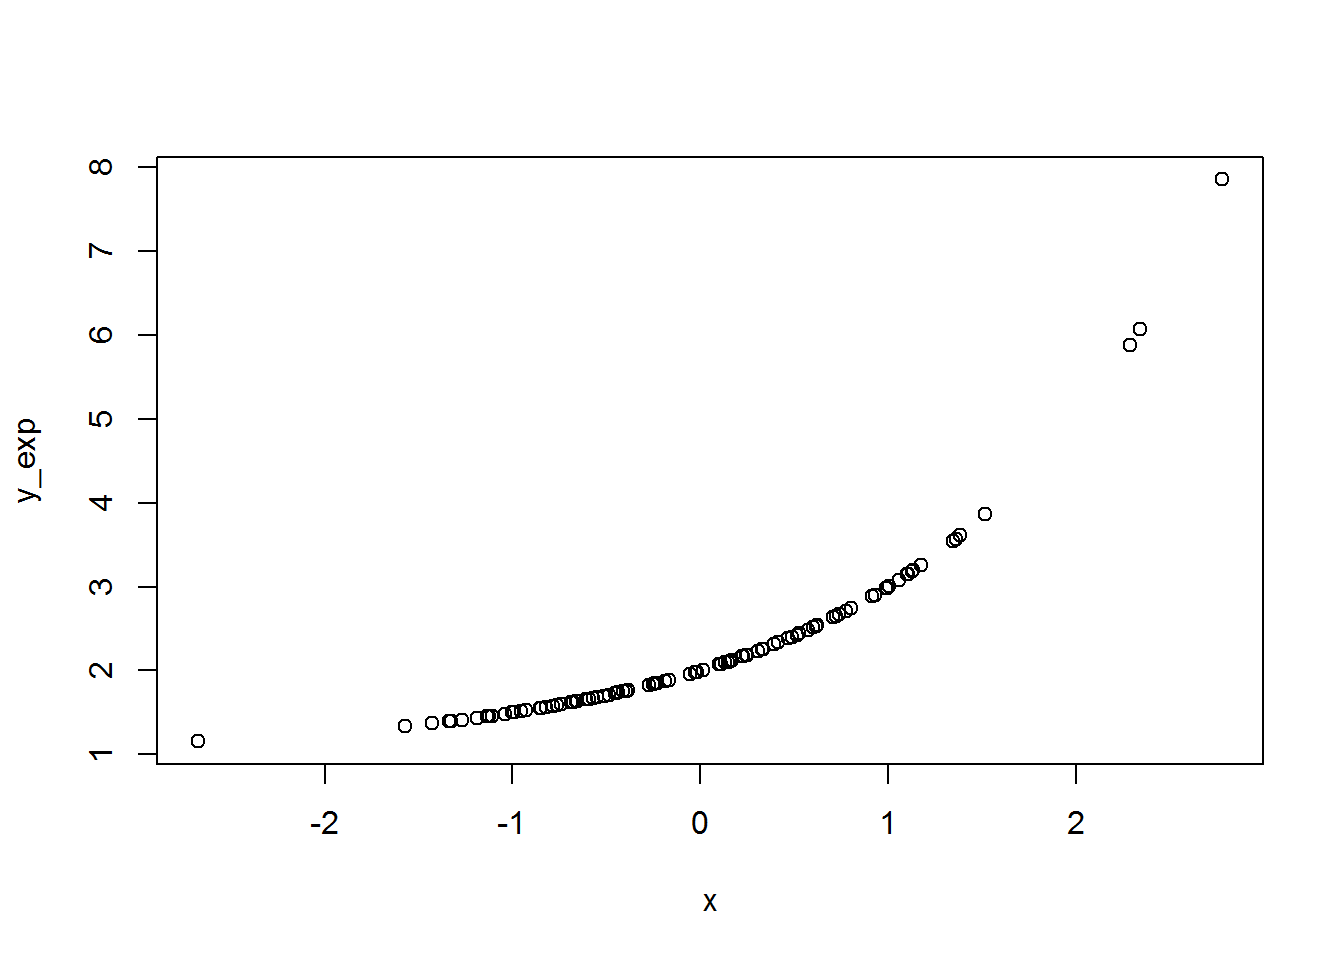
\includegraphics{introR_files/figure-latex/unnamed-chunk-9-1} 

}

\caption{figura de una curva exponencial.}\label{fig:unnamed-chunk-9}
\end{figure}

\begin{Shaded}
\begin{Highlighting}[]
\NormalTok{z <-}\StringTok{ }\NormalTok{(x}\OperatorTok{-}\KeywordTok{mean}\NormalTok{(x))}\OperatorTok{/}\KeywordTok{sd}\NormalTok{(x)  }\CommentTok{# see also 'scale'}

\KeywordTok{mean}\NormalTok{(z) }\CommentTok{# la media}
\end{Highlighting}
\end{Shaded}

\begin{verbatim}
## [1] -8.626455e-18
\end{verbatim}

\begin{Shaded}
\begin{Highlighting}[]
\KeywordTok{sd}\NormalTok{(y_exp) }\CommentTok{# la desviacióm}
\end{Highlighting}
\end{Shaded}

\begin{verbatim}
## [1] 0.9095358
\end{verbatim}

\hypertarget{inspeccionando-vectores}{%
\section{Inspeccionando vectores}\label{inspeccionando-vectores}}

Las siguientes funciones, sirven para inspeccionar el contenido de un vector:

\begin{Shaded}
\begin{Highlighting}[]
\KeywordTok{length}\NormalTok{(x)}
\KeywordTok{table}\NormalTok{(x)  }\CommentTok{# ¡muy importante! Cuenta cuantos valores de cada numero}
\KeywordTok{summary}\NormalTok{(y)}
\KeywordTok{head}\NormalTok{(x)}
\KeywordTok{tail}\NormalTok{(x)}
\end{Highlighting}
\end{Shaded}

Para seleccionar elementos de un vector se usa el corchete {[}{]}. Pero, a diferencia de lo que ocurre con las tablas, como los vectores son objetos unidimensionales, no se usa coma. Obviamente, el corchete sigue admitiendo no solo los índices de los elementos que se quieren extraer, sino que además permite utilizar condiciones lógicas.

\begin{Shaded}
\begin{Highlighting}[]
\NormalTok{x[}\DecValTok{1}\OperatorTok{:}\DecValTok{33}\NormalTok{]}
\NormalTok{x[}\KeywordTok{c}\NormalTok{(}\DecValTok{1}\NormalTok{,}\DecValTok{3}\NormalTok{)]}
\NormalTok{x[x }\OperatorTok{>}\StringTok{ }\FloatTok{1.5}\NormalTok{]}
\NormalTok{x[}\DecValTok{3}\OperatorTok{:}\DecValTok{1}\NormalTok{]}
\NormalTok{x[}\OperatorTok{-}\NormalTok{(}\DecValTok{1}\OperatorTok{:}\DecValTok{2}\NormalTok{)]}
\NormalTok{x[}\OperatorTok{-}\KeywordTok{length}\NormalTok{(x)]}
\end{Highlighting}
\end{Shaded}

\hypertarget{matrices}{%
\chapter{Matrices}\label{matrices}}

Las matrices son el sigiente paso luego de los vectores. Las matrices son muy útiles en calculos algebraicos. Ls matrices se crean dimensionando un vector con la funcion dim o con la funcion matrix. Veamos algúnos ejemplos:

\begin{Shaded}
\begin{Highlighting}[]
\CommentTok{###################}
\CommentTok{# Creating Matrices: dim and matrix functions}
\NormalTok{value <-}\StringTok{ }\KeywordTok{rnorm}\NormalTok{(}\DecValTok{12}\NormalTok{)}
\KeywordTok{dim}\NormalTok{(value) <-}\StringTok{ }\KeywordTok{c}\NormalTok{(}\DecValTok{4}\NormalTok{,}\DecValTok{3}\NormalTok{)}
\NormalTok{value}
\end{Highlighting}
\end{Shaded}

\begin{verbatim}
##            [,1]        [,2]       [,3]
## [1,] -0.3618069  1.56467517 -1.1430813
## [2,]  0.6661578 -0.94720179 -1.2218039
## [3,] -0.5214987 -0.05357234 -1.6527820
## [4,] -0.3306759 -1.53352221  0.2238258
\end{verbatim}

\begin{Shaded}
\begin{Highlighting}[]
\KeywordTok{dim}\NormalTok{(value) <-}\StringTok{ }\OtherTok{NULL}
\KeywordTok{matrix}\NormalTok{(value,}\DecValTok{2}\NormalTok{,}\DecValTok{3}\NormalTok{)}
\end{Highlighting}
\end{Shaded}

\begin{verbatim}
##            [,1]       [,2]       [,3]
## [1,] -0.3618069 -0.5214987  1.5646752
## [2,]  0.6661578 -0.3306759 -0.9472018
\end{verbatim}

\begin{Shaded}
\begin{Highlighting}[]
\KeywordTok{matrix}\NormalTok{(value,}\DecValTok{2}\NormalTok{,}\DecValTok{3}\NormalTok{,}\DataTypeTok{byrow=}\NormalTok{T)}
\end{Highlighting}
\end{Shaded}

\begin{verbatim}
##            [,1]      [,2]       [,3]
## [1,] -0.3618069 0.6661578 -0.5214987
## [2,] -0.3306759 1.5646752 -0.9472018
\end{verbatim}

\begin{Shaded}
\begin{Highlighting}[]
\CommentTok{# Creating Matrices: rbind and cbind functions}
\NormalTok{value <-}\StringTok{ }\KeywordTok{matrix}\NormalTok{(}\KeywordTok{rnorm}\NormalTok{(}\DecValTok{6}\NormalTok{),}\DecValTok{2}\NormalTok{,}\DecValTok{3}\NormalTok{,}\DataTypeTok{byrow=}\NormalTok{T)}
\NormalTok{value2 <-}\StringTok{ }\KeywordTok{rbind}\NormalTok{(value,}\KeywordTok{c}\NormalTok{(}\DecValTok{1}\NormalTok{,}\DecValTok{1}\NormalTok{,}\DecValTok{2}\NormalTok{))}
\NormalTok{value2}
\end{Highlighting}
\end{Shaded}

\begin{verbatim}
##           [,1]       [,2]       [,3]
## [1,] 0.6895265  0.5216871 -0.9152526
## [2,] 0.9548875 -1.4039183 -1.0740219
## [3,] 1.0000000  1.0000000  2.0000000
\end{verbatim}

\begin{Shaded}
\begin{Highlighting}[]
\NormalTok{value3 <-}\StringTok{ }\KeywordTok{cbind}\NormalTok{(value2,}\KeywordTok{c}\NormalTok{(}\DecValTok{1}\NormalTok{,}\DecValTok{1}\NormalTok{,}\DecValTok{2}\NormalTok{))}
\end{Highlighting}
\end{Shaded}

Las matrices son objetos que parecen tablas sin serlo en forma estricta.

\hypertarget{tablas}{%
\chapter{Tablas}\label{tablas}}

Las tablas en R se conocen como Data Frames.

Muy frecuentemente, los datos se disponen en tablas: las hojas de cálculo, las bases de datos, los ficheros csv, etc. contienen, esencialmente, tablas. Además, casi todos los métodos estadísticos (p.e., la regresión lineal) operan sobre información organizada en tablas. Como consecuencia, gran parte del día a día del trabajo con R consiste en manipular tablas de datos para darles el formato necesario para acabar analizándolos estadística o gráficamente.

Las hojas de cálculo son herramientas que prácticamente todos hemos usado para manipular tablas de datos. Sin embargo R y R studio no permiten la flexibilidad de manejar tablas con el mouse. Asi que hay que aprender algunos comandos basicos para manipular e indexar.

\hypertarget{crear-data-frames}{%
\section{Crear Data Frames}\label{crear-data-frames}}

Para practicar y como ejemplo, usaremos una tabla que viene por defecto con R. Se trata de la tabla iris3. Esta tiene columnas que contienen cuatro características métricas de cada especie de flor: la longitud y la anchura de sus pétalos y sépalos; y la especie: setosa, versicolor o virgínica, a la que pertenecen. De momento y hasta que aprendamos cómo importar datos de fuentes externas, utilizaremos este y otros conjuntos de datos de ejemplo que incluye R.

Ya que es impráctico mostrar tablas enteras en la consola, sobre todo cuando son grandes. Para mostrar solo parte de ellas, hay algunas funciones útiles para inspeccionar tablas (y, como veremos más adelante, no solo tablas), esta son:

\begin{Shaded}
\begin{Highlighting}[]
\KeywordTok{str}\NormalTok{ (iris)        }\CommentTok{# "representación textual" del objeto}
\KeywordTok{class}\NormalTok{ (iris)      }\CommentTok{# "representación de la clase" del objeto}
\KeywordTok{head}\NormalTok{ (iris)    }\CommentTok{# primeras seis filas}
\KeywordTok{tail}\NormalTok{ (iris)    }\CommentTok{# últimas seis filas}
\KeywordTok{dim}\NormalTok{ (iris)     }\CommentTok{# filas x columnas}
\KeywordTok{colnames}\NormalTok{ (iris)  }\CommentTok{# nombre de sus columnas}
\KeywordTok{summary}\NormalTok{ (iris)  }\CommentTok{# resumen estadístico de las columnas}
\end{Highlighting}
\end{Shaded}

\hypertarget{indexar-data-frames}{%
\section{Indexar data frames}\label{indexar-data-frames}}

Las tablas se indexan usando el corchete {[}{]} y este debe ir separado por una coma {[},{]} donde el primer valor representa las filas y el segundo las columnas, siempre en ese orden. Por ejemplo:

\begin{Shaded}
\begin{Highlighting}[]
\NormalTok{iris[}\DecValTok{1}\OperatorTok{:}\DecValTok{5}\NormalTok{,] }\CommentTok{# muestra las 5 primeras filas}
\NormalTok{iris[,}\DecValTok{1}\OperatorTok{:}\DecValTok{3}\NormalTok{] }\CommentTok{# muestra las 3 primeras columnas}
\NormalTok{iris[}\DecValTok{25}\NormalTok{,}\DecValTok{4}\NormalTok{] }\CommentTok{# muestra el dato de la fila 25 y columna 4 }

\CommentTok{# los corchetes tambien admiten los nombres de las columnas}
\NormalTok{iris[, }\StringTok{"Species"}\NormalTok{] }

\CommentTok{## Usando el $ en las tablas}
\CommentTok{# Pero se usa mas habitualmente (porque es más rápido y más legible) iris$Species en lugar de iris[, "Species"]}
\NormalTok{iris}\OperatorTok{$}\NormalTok{Species }
\end{Highlighting}
\end{Shaded}

El corchete también permite seleccionar filas mediante condiciones lógicas. Por ejemplo seleccionemos de la tabla de iris las que corresponden a la especie setosa:

\begin{Shaded}
\begin{Highlighting}[]
\NormalTok{iris[iris}\OperatorTok{$}\NormalTok{Species }\OperatorTok{==}\StringTok{ "setosa"}\NormalTok{,]}
\end{Highlighting}
\end{Shaded}

\begin{quote}
\hypertarget{ejercicio}{%
\subsection{Ejercicio:}\label{ejercicio}}

Selecciona las filas de iris cuya longitud del pétalo sea mayor que 4.
\end{quote}

\hypertarget{crear-una-columna-nueva}{%
\section{Crear una columna nueva}\label{crear-una-columna-nueva}}

Lo mas practico es usar el nombre de la tabla seguido de \$ y el nombre de la nueva columna. Por ejemplo creemos la columna raiz cuadrada de la longitud del petalo

\begin{Shaded}
\begin{Highlighting}[]
\NormalTok{iris}\OperatorTok{$}\NormalTok{raiz_petalo <-}\StringTok{ }\KeywordTok{sqrt}\NormalTok{ (iris}\OperatorTok{$}\NormalTok{Petal.Length) }\CommentTok{# sqrt es la raiz cuadrada.}
\end{Highlighting}
\end{Shaded}

Tengan en cuenta que:

\begin{itemize}
\tightlist
\item
  agregar una columna que ya existe la reemplaza,
\item
  agregar una columna que no existe la crea y
\item
  asignar NULL a una columna existente la elimina.
\end{itemize}

\hypertarget{visualizar-la-tabla-graficamente}{%
\section{Visualizar la tabla graficamente}\label{visualizar-la-tabla-graficamente}}

\hypertarget{como-histograma}{%
\subsection{Como histograma}\label{como-histograma}}

A veces es mucho más informativa una representación visual de los datos. La manera más rápida (y recomendada) de hacerse una idea de la distribución de los datos de una columna numérica es usando histogramas. En R, para representar el histograma de la columna Sepal.Width de iris se puede hacer:

\begin{Shaded}
\begin{Highlighting}[]
\KeywordTok{hist}\NormalTok{(iris}\OperatorTok{$}\NormalTok{Sepal.Width)}
\end{Highlighting}
\end{Shaded}

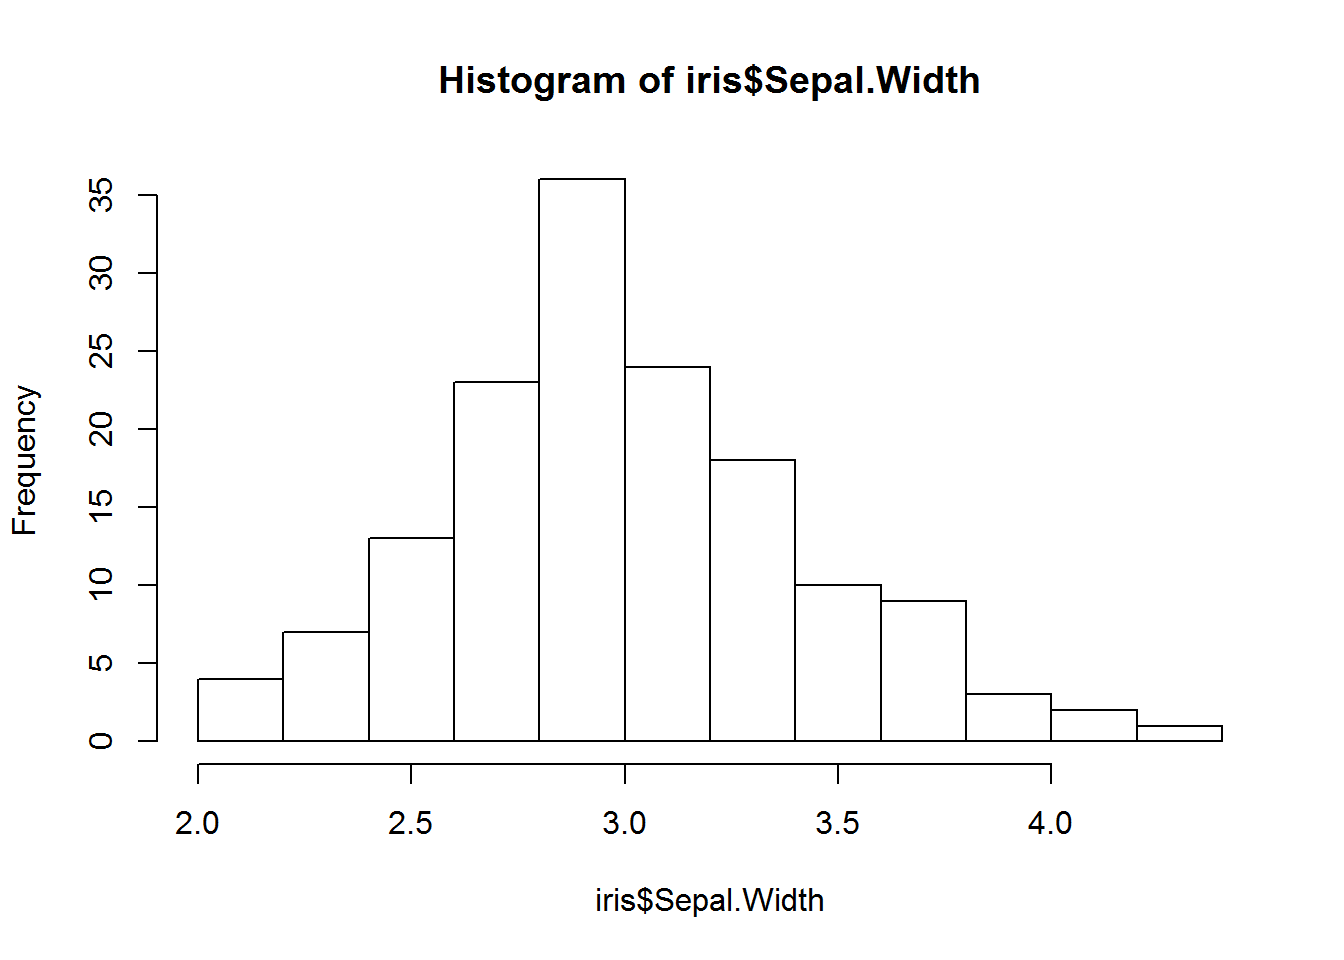
\includegraphics{introR_files/figure-latex/unnamed-chunk-17-1.pdf}

\begin{Shaded}
\begin{Highlighting}[]
\CommentTok{#### y para editar el grafico se especifican parametros adicionales}
\KeywordTok{hist}\NormalTok{(iris}\OperatorTok{$}\NormalTok{Sepal.Width, }\DataTypeTok{main =} \StringTok{"iris: histograma de la anchura de los sépalos"}\NormalTok{,}
      \DataTypeTok{xlab =} \StringTok{"anchura del sépalo"}\NormalTok{, }\DataTypeTok{ylab =} \StringTok{"frecuencia"}\NormalTok{,}
      \DataTypeTok{col =} \StringTok{"steelblue"}\NormalTok{)}
\end{Highlighting}
\end{Shaded}

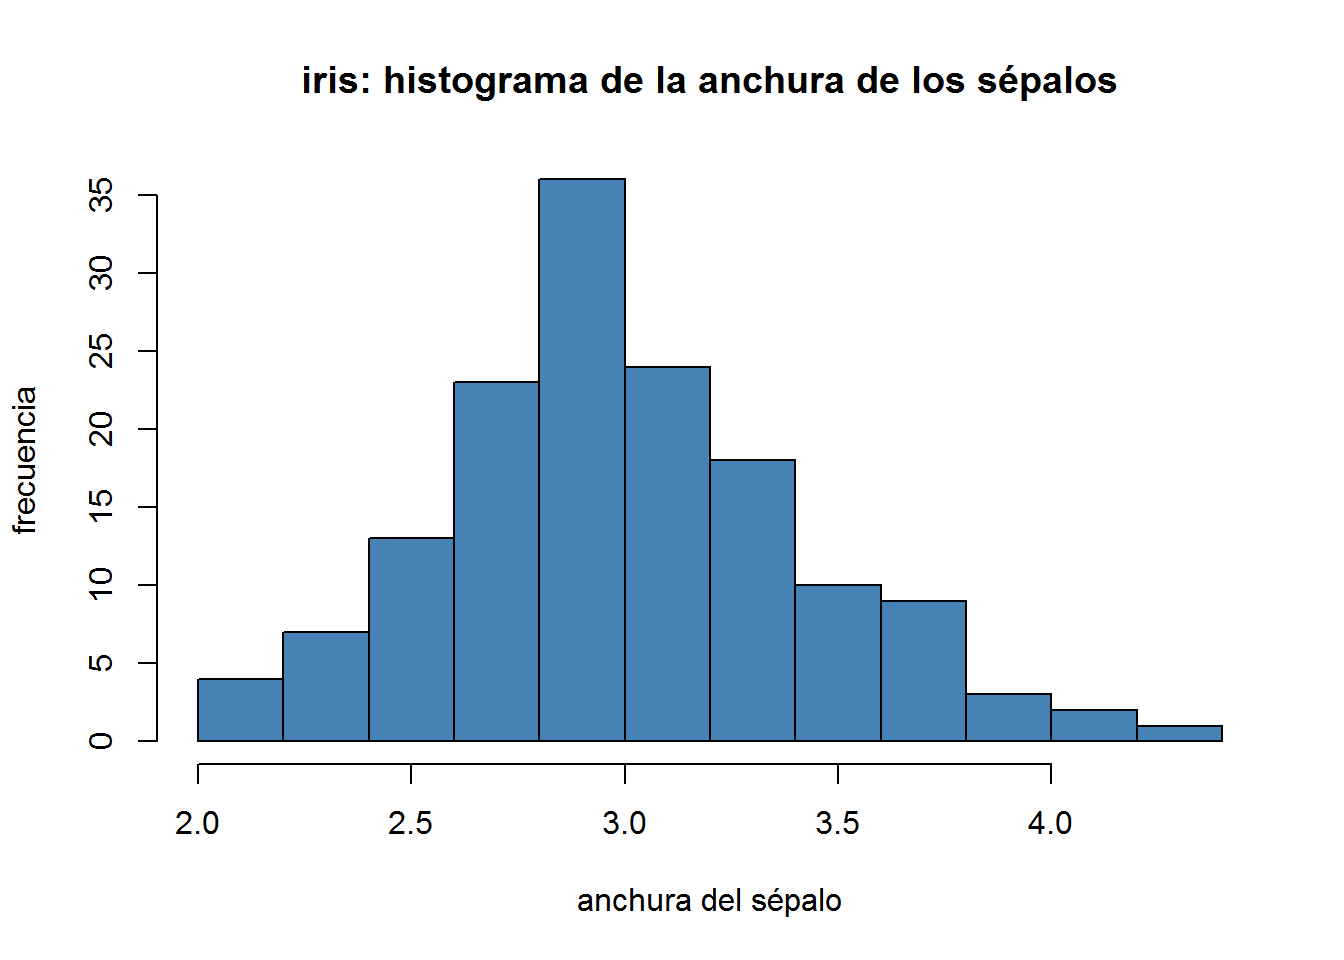
\includegraphics{introR_files/figure-latex/unnamed-chunk-17-2.pdf}

\hypertarget{como-dos-variables-numericas}{%
\subsection{Como dos variables numericas}\label{como-dos-variables-numericas}}

Por ejemplo representemos la lomgitud del sepalo versus el petalo.

\begin{Shaded}
\begin{Highlighting}[]
\KeywordTok{plot}\NormalTok{(iris}\OperatorTok{$}\NormalTok{Sepal.Length, iris}\OperatorTok{$}\NormalTok{Petal.Length)}
\end{Highlighting}
\end{Shaded}

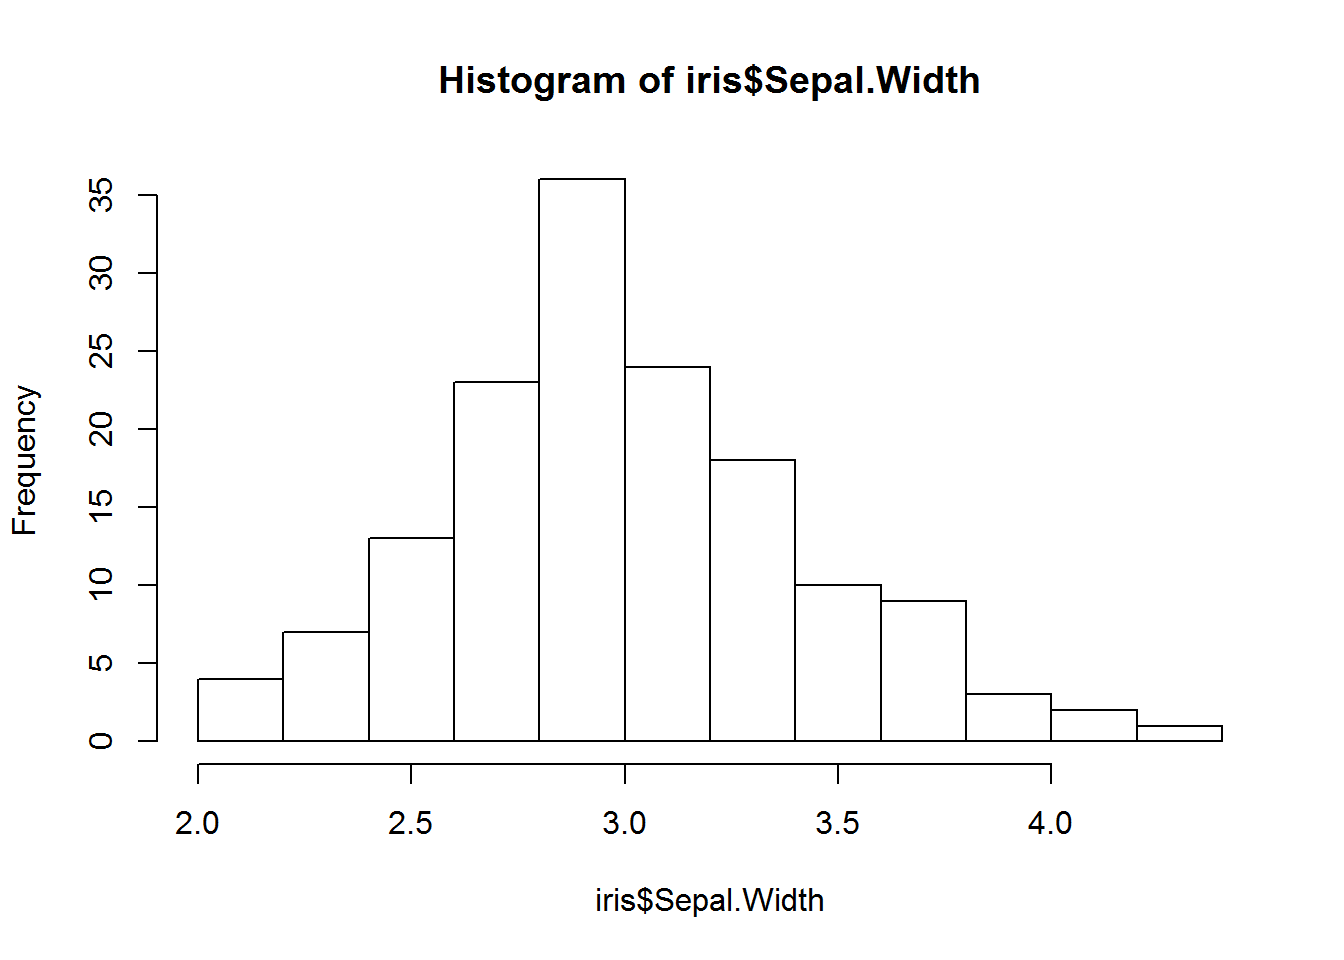
\includegraphics{introR_files/figure-latex/unnamed-chunk-18-1.pdf}

\hypertarget{diagrama-de-caja-boxplots}{%
\subsection{Diagrama de caja (boxplots)}\label{diagrama-de-caja-boxplots}}

Los diagramas de cajas (boxplot) estudian la distribución de una variable continua en función de una variable categórica. Están emparentados con los histogramas porque resumen la distribución de una variable continua. Para ello utilizan una representación todavía mas esquemática que la de un histograma: una caja y unos segmentos que acotan las regiones donde la variable continua concentra el grueso de las observaciones.

Por ejemplo, podemos estudiar la distribución de la anchura del sépalo en iris en función de la especie usando diagramas de cajas así:

\begin{Shaded}
\begin{Highlighting}[]
\KeywordTok{boxplot}\NormalTok{(iris}\OperatorTok{$}\NormalTok{Sepal.Width }\OperatorTok{~}\StringTok{ }\NormalTok{iris}\OperatorTok{$}\NormalTok{Species, }\DataTypeTok{col =} \StringTok{"gray"}\NormalTok{,}
        \DataTypeTok{main =} \StringTok{"Especies de iris}\CharTok{\textbackslash{}n}\StringTok{según la anchura del sépalo"}\NormalTok{)}
\end{Highlighting}
\end{Shaded}

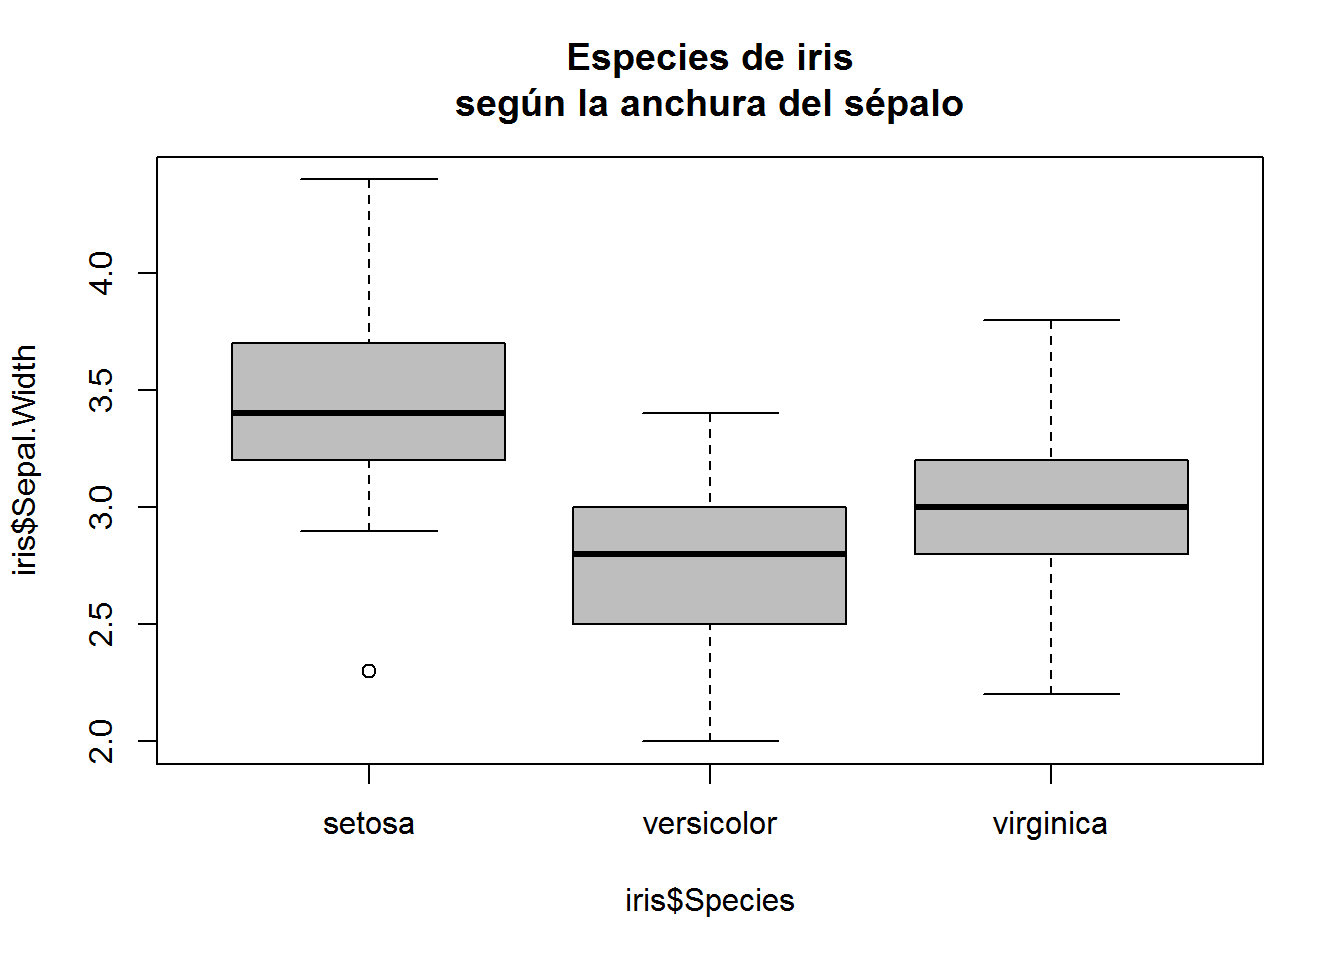
\includegraphics{introR_files/figure-latex/unnamed-chunk-19-1.pdf}

La notación y \textasciitilde{} x es muy común en R y significa que vas a hacer algo con y en función de x; en este caso, algo es un diagrama de cajas. Cuando construyamos modelos, querremos entender la variable objetivo y en función de una o más variables predictoras y volveremos a hacer uso de esa notación.

\hypertarget{creaciuxf3n-y-e-indexaciuxf3n-de-listas}{%
\chapter{Creación y e indexación de listas}\label{creaciuxf3n-y-e-indexaciuxf3n-de-listas}}

Las tablas son contenedores de información estructurada: las columnas son del mismo tipo, todas tienen la misma longitud, etc. Gran parte de los datos con los que se trabaja habitualmente son estructurados, palabra que, en la jerga, significa que admiten una representación tabular.

Sin embargo, cada vez es más habitual trabajar directamente con información desestructurada. Particularmente, en ciencia de datos. Eso justifica el uso de las listas, que pueden definirse como contenedores genéricos de información desestructurada.

Las listas son objetos muy versatiles que mezclan varias cosas y sirven como contenedores genericos de dstos e informacón. Estas son una ventaja de R, sobre otros lenguajes como Python que no las tienen. Pero pueden llegar a ser objetos complejos dificiles de entender y visualizar.

\begin{Shaded}
\begin{Highlighting}[]
\NormalTok{a <-}\StringTok{ }\KeywordTok{c}\NormalTok{(}\DecValTok{1}\NormalTok{,}\DecValTok{2}\NormalTok{,}\DecValTok{3}\NormalTok{,}\DecValTok{4}\NormalTok{,}\DecValTok{5}\NormalTok{,}\DecValTok{6}\NormalTok{,}\DecValTok{7}\NormalTok{) }\CommentTok{# vector numerico}
\NormalTok{b <-}\StringTok{ }\KeywordTok{c}\NormalTok{(}\StringTok{"Casa"}\NormalTok{, }\StringTok{"Carro"}\NormalTok{, }\StringTok{"Beca"}\NormalTok{) }\CommentTok{# vector alfanumerico}

\NormalTok{florecitas <-}\StringTok{ }\NormalTok{iris[}\DecValTok{3}\OperatorTok{:}\DecValTok{25}\NormalTok{,}\DecValTok{2}\OperatorTok{:}\DecValTok{5}\NormalTok{] }\CommentTok{#data frame}

\NormalTok{lista1 <-}\StringTok{ }\KeywordTok{list}\NormalTok{(a, b, florecitas)}
\end{Highlighting}
\end{Shaded}

las listas disponen de un operador para extraer elementos, los dobles corchetes, {[}{[}{]}{]}, que funcionan de manera parecida y analoga a \$.

\begin{Shaded}
\begin{Highlighting}[]
\NormalTok{lista1[[}\DecValTok{2}\NormalTok{]] }\CommentTok{# extrae el objeto b}
\end{Highlighting}
\end{Shaded}

\begin{verbatim}
## [1] "Casa"  "Carro" "Beca"
\end{verbatim}

\begin{Shaded}
\begin{Highlighting}[]
\NormalTok{lista1[[}\DecValTok{3}\NormalTok{]] [,}\DecValTok{4}\NormalTok{] }\CommentTok{# extrae la columna 4 del objeto 3}
\end{Highlighting}
\end{Shaded}

\begin{verbatim}
##  [1] setosa setosa setosa setosa setosa setosa setosa setosa setosa
## [10] setosa setosa setosa setosa setosa setosa setosa setosa setosa
## [19] setosa setosa setosa setosa setosa
## Levels: setosa versicolor virginica
\end{verbatim}

\hypertarget{creaciuxf3n-de-funciones}{%
\chapter{Creación de Funciones}\label{creaciuxf3n-de-funciones}}

Esta sección, por su importancia, pertenece propiamente a la sección de programación. La creación de funciones en lo que sigue del curso es fundemental y, presenta la gran versatilidad de un lenguaje de programación.

Creemos una función que opera sobre un vector que vamos a llamar x

\begin{Shaded}
\begin{Highlighting}[]
\NormalTok{media <-}\StringTok{ }\ControlFlowTok{function}\NormalTok{(x)\{     }\CommentTok{# inicio de la funcion}
\NormalTok{ longitud <-}\StringTok{ }\KeywordTok{length}\NormalTok{(x)}
\NormalTok{ suma <-}\StringTok{ }\KeywordTok{sum}\NormalTok{(x)}
 \KeywordTok{return}\NormalTok{ (suma }\OperatorTok{/}\StringTok{ }\NormalTok{longitud) }\CommentTok{# devuelve el resultado de la media}
\NormalTok{\}                         }\CommentTok{# final de la funcion}


\CommentTok{# creemos un vector}
\NormalTok{vector1 <-}\StringTok{ }\KeywordTok{rnorm}\NormalTok{ (}\DecValTok{100}\NormalTok{) }\CommentTok{# 100 datos al azar de la distribucion normal}

\CommentTok{# apliquemos la funcion al vector}
\KeywordTok{media}\NormalTok{(vector1)}
\end{Highlighting}
\end{Shaded}

\begin{verbatim}
## [1] 0.06964508
\end{verbatim}

\hypertarget{creaciuxf3n-de-bucles}{%
\chapter{Creación de bucles}\label{creaciuxf3n-de-bucles}}

En la programación en R es habitual construir loops o bucles dentro de los cuales se va modificando el valor de una expresión. Los bucles más habituales en R comienzan con for. Su sintaxis es

for (var in vector)\{
\# expresión que se repite
\}

Ejemplo: construyamos un bucle que repite la impresion de un nombre 10 veces

\begin{Shaded}
\begin{Highlighting}[]
\ControlFlowTok{for}\NormalTok{ (i }\ControlFlowTok{in} \DecValTok{1}\OperatorTok{:}\DecValTok{10}\NormalTok{)\{     }\CommentTok{# variable i en un vector de 1 a 10}
  \KeywordTok{print}\NormalTok{ (}\StringTok{"Carlos"}\NormalTok{)   }\CommentTok{# expresión que se repite}
\NormalTok{\}                    }\CommentTok{# final del bucle}
\end{Highlighting}
\end{Shaded}

\begin{verbatim}
## [1] "Carlos"
## [1] "Carlos"
## [1] "Carlos"
## [1] "Carlos"
## [1] "Carlos"
## [1] "Carlos"
## [1] "Carlos"
## [1] "Carlos"
## [1] "Carlos"
## [1] "Carlos"
\end{verbatim}

Hagamos un bucle mas interesante que simula datos de pesencia ausencia obtenidos al azar (con probabilidad 0.5) de la distibucion binomial, para un estudio de ocupacion con 15 sitios y cuatro visitas repetidas a cada sitio.

\begin{Shaded}
\begin{Highlighting}[]
\NormalTok{sitios  <-}\StringTok{ }\DecValTok{15}
\NormalTok{visitas <-}\StringTok{ }\DecValTok{4}
\NormalTok{datos <-}\StringTok{ }\KeywordTok{matrix}\NormalTok{(}\OtherTok{NA}\NormalTok{, }\DecValTok{15}\NormalTok{,}\DecValTok{4}\NormalTok{) }\CommentTok{# matriz vacia donde vamos a poner los datos}

\ControlFlowTok{for}\NormalTok{ (i }\ControlFlowTok{in} \DecValTok{1}\OperatorTok{:}\NormalTok{sitios)\{     }\CommentTok{# variable i en un vector de 1 a 10}
\NormalTok{  y <-}\StringTok{ }\KeywordTok{rbinom}\NormalTok{(visitas, }\DecValTok{1}\NormalTok{, }\FloatTok{0.5}\NormalTok{) }\CommentTok{# 0.5 es la probabilidad}
\NormalTok{  datos [i,] <-}\StringTok{ }\NormalTok{y}
\NormalTok{\}                    }

\NormalTok{datos}
\end{Highlighting}
\end{Shaded}

\begin{verbatim}
##       [,1] [,2] [,3] [,4]
##  [1,]    0    1    1    1
##  [2,]    0    1    0    1
##  [3,]    1    1    1    0
##  [4,]    0    0    1    1
##  [5,]    0    1    0    1
##  [6,]    0    1    1    1
##  [7,]    1    1    0    0
##  [8,]    1    0    1    1
##  [9,]    0    1    0    1
## [10,]    1    1    1    0
## [11,]    0    0    1    1
## [12,]    0    0    1    1
## [13,]    1    0    1    1
## [14,]    1    0    0    1
## [15,]    0    0    1    1
\end{verbatim}

\begin{quote}
\hypertarget{ejercicio-1}{%
\subsection{Ejercicio:}\label{ejercicio-1}}

Crear una matriz de datos simulados, de un estudio donde se cuentan renacuajos en 20 sitios con cinco visitas repetidas a cada sitio.
\end{quote}

\hypertarget{convirtamolo-en-funciuxf3n}{%
\section{Convirtamolo en función}\label{convirtamolo-en-funciuxf3n}}

\begin{Shaded}
\begin{Highlighting}[]
\NormalTok{genera_datos <-}\StringTok{ }\ControlFlowTok{function}\NormalTok{(}\DataTypeTok{sitios=}\DecValTok{15}\NormalTok{, }\DataTypeTok{visitas=}\DecValTok{4}\NormalTok{, }\DataTypeTok{probabilidad=}\FloatTok{0.5}\NormalTok{) \{}
\NormalTok{  datos <-}\StringTok{ }\KeywordTok{matrix}\NormalTok{(}\OtherTok{NA}\NormalTok{, sitios, visitas) }\CommentTok{# matriz vacia donde vamos a poner los datos}
  
  \ControlFlowTok{for}\NormalTok{ (i }\ControlFlowTok{in} \DecValTok{1}\OperatorTok{:}\NormalTok{sitios)\{     }\CommentTok{# variable i }
\NormalTok{    y <-}\StringTok{ }\KeywordTok{rbinom}\NormalTok{(visitas, }\DecValTok{1}\NormalTok{, probabilidad) }\CommentTok{# dados guardados en y}
\NormalTok{    datos [i,] <-}\StringTok{ }\NormalTok{y       }\CommentTok{# y pasa a la fila i de la tabla de datos}
\NormalTok{  \}  }
  \KeywordTok{return}\NormalTok{(datos) }\CommentTok{# muestra los datos al finalizar el bucle}
\NormalTok{\}                  }


\CommentTok{# llamemos la funcion }
\KeywordTok{genera_datos}\NormalTok{() }\CommentTok{#con los valores por defecto}
\end{Highlighting}
\end{Shaded}

\begin{verbatim}
##       [,1] [,2] [,3] [,4]
##  [1,]    0    1    1    1
##  [2,]    1    0    1    1
##  [3,]    1    1    0    0
##  [4,]    1    0    1    0
##  [5,]    0    0    0    1
##  [6,]    0    0    1    1
##  [7,]    1    0    0    1
##  [8,]    1    1    0    1
##  [9,]    0    0    0    0
## [10,]    0    1    0    0
## [11,]    1    0    0    0
## [12,]    0    0    1    1
## [13,]    0    1    0    1
## [14,]    1    1    0    1
## [15,]    1    1    1    1
\end{verbatim}

\begin{Shaded}
\begin{Highlighting}[]
\KeywordTok{genera_datos}\NormalTok{(}\DecValTok{30}\NormalTok{, }\DecValTok{6}\NormalTok{, }\FloatTok{0.5}\NormalTok{) }\CommentTok{# con 30 sitios, 6 visitas repetidas y probabilidad 0.5}
\end{Highlighting}
\end{Shaded}

\begin{verbatim}
##       [,1] [,2] [,3] [,4] [,5] [,6]
##  [1,]    1    1    0    0    0    1
##  [2,]    1    1    1    1    1    0
##  [3,]    0    0    1    1    1    1
##  [4,]    0    1    1    1    0    0
##  [5,]    0    0    1    1    0    1
##  [6,]    1    0    0    0    1    0
##  [7,]    0    1    0    0    1    1
##  [8,]    1    1    1    0    1    0
##  [9,]    0    0    0    0    1    1
## [10,]    1    0    1    1    0    1
## [11,]    1    1    0    1    1    1
## [12,]    0    1    0    0    0    1
## [13,]    1    0    1    1    0    0
## [14,]    0    1    0    1    0    0
## [15,]    1    0    1    0    0    0
## [16,]    0    1    1    0    0    1
## [17,]    1    1    0    1    1    0
## [18,]    1    0    0    0    0    1
## [19,]    1    1    0    0    1    1
## [20,]    1    0    1    1    1    0
## [21,]    0    1    1    0    1    0
## [22,]    0    1    0    1    1    1
## [23,]    1    0    0    0    1    0
## [24,]    1    0    1    1    1    1
## [25,]    1    1    0    0    0    1
## [26,]    0    0    0    1    0    1
## [27,]    0    1    1    0    1    0
## [28,]    1    0    1    0    1    0
## [29,]    1    1    0    1    0    1
## [30,]    1    0    1    1    1    0
\end{verbatim}

\hypertarget{modelos-en-r}{%
\chapter{Modelos en R}\label{modelos-en-r}}

Los modelos son una simplificación y abstracción de un sistema real que nos permite entender un proceso y/o sus resultados. Adicionalmente permiten entender como interactuan o se afectan los parametros si variamos algo dentro del modelo.

\hypertarget{modelo-de-la-media}{%
\section{Modelo de la media}\label{modelo-de-la-media}}

Aunque este primer modelo no es un modelo como tal, el siguiente código nos permite entender como el tamaño de la muestra afecta la distribución de la media. Para esto usaremos el set de datos iris de R y la columna largo del pétalo. Lo que haremos será extraer al azar un numero (n) de valores del vector largo del pétalo y calcular la media cien veces. Con estos valores construiremos un histograma.

Haremos una comparación grafica de la forma del histograma con la media (original) del vector largo del pétalo, el cual representaremos con color azul.

\begin{Shaded}
\begin{Highlighting}[]
\KeywordTok{str}\NormalTok{(iris)}
\end{Highlighting}
\end{Shaded}

\begin{verbatim}
## 'data.frame':    150 obs. of  5 variables:
##  $ Sepal.Length: num  5.1 4.9 4.7 4.6 5 5.4 4.6 5 4.4 4.9 ...
##  $ Sepal.Width : num  3.5 3 3.2 3.1 3.6 3.9 3.4 3.4 2.9 3.1 ...
##  $ Petal.Length: num  1.4 1.4 1.3 1.5 1.4 1.7 1.4 1.5 1.4 1.5 ...
##  $ Petal.Width : num  0.2 0.2 0.2 0.2 0.2 0.4 0.3 0.2 0.2 0.1 ...
##  $ Species     : Factor w/ 3 levels "setosa","versicolor",..: 1 1 1 1 1 1 1 1 1 1 ...
\end{verbatim}

\begin{Shaded}
\begin{Highlighting}[]
\NormalTok{iter <-}\StringTok{ }\DecValTok{100} \CommentTok{# Numero de iteraciones}
\NormalTok{n <-}\StringTok{ }\DecValTok{1} \CommentTok{# numero de datos que muestreo. Variar hasta 150}
\NormalTok{means <-}\StringTok{ }\KeywordTok{rep}\NormalTok{(}\OtherTok{NA}\NormalTok{, iter) }\CommentTok{# aca almaceno las medias de cada iteracion}

\ControlFlowTok{for}\NormalTok{ (i }\ControlFlowTok{in} \DecValTok{1}\OperatorTok{:}\NormalTok{iter)\{}
\NormalTok{  d <-}\StringTok{ }\KeywordTok{sample}\NormalTok{(iris}\OperatorTok{$}\NormalTok{Petal.Length, n) }\CommentTok{# sample toma n (1) datos }
\NormalTok{  means[i] <-}\StringTok{ }\KeywordTok{mean}\NormalTok{(d) }\CommentTok{# saca la media y guarda en means }
\NormalTok{\}}

\KeywordTok{hist}\NormalTok{(means)}
\KeywordTok{abline}\NormalTok{(}\DataTypeTok{v=}\KeywordTok{mean}\NormalTok{(iris}\OperatorTok{$}\NormalTok{Petal.Length), }\DataTypeTok{lty=}\DecValTok{2}\NormalTok{, }\DataTypeTok{lwd=}\DecValTok{3}\NormalTok{, }\DataTypeTok{col=}\StringTok{"blue"}\NormalTok{)}
\end{Highlighting}
\end{Shaded}

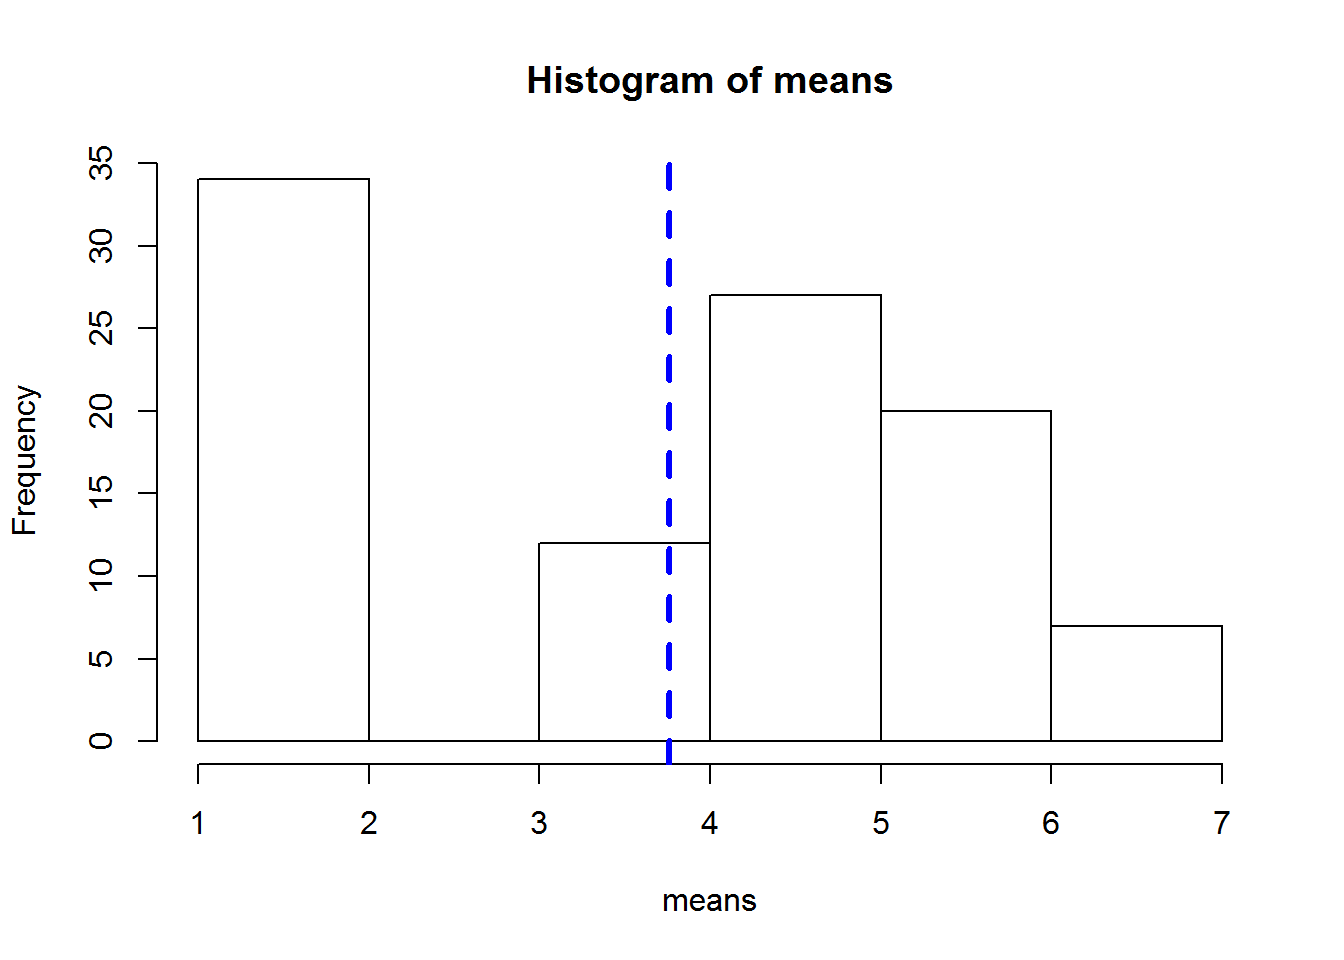
\includegraphics{introR_files/figure-latex/unnamed-chunk-26-1.pdf}

Ahora repitamos el mismo código 10 veces para ver como varia el histograma, ya que estamos seleccioando valores al azar.

Como siguiente paso cambiemos el valor de n a dos (n \textless- 2), luego a tres, luego cuatro, cinco\ldots{} etc.

\begin{quote}
\hypertarget{ejercicio-1-1}{%
\subsection{Ejercicio 1}\label{ejercicio-1-1}}

Discuta como varia la forma del histograma en la medida en que el valor de n aumenta.
\end{quote}

\begin{quote}
\hypertarget{ejercicio-2}{%
\subsection{Ejercicio 2}\label{ejercicio-2}}

Convierta el código en una funcion de forma tal que pueda variar el valor de n para producir las graficas en una sola linea.
\end{quote}

\hypertarget{modelo-de-regresiuxf3n-lineal}{%
\chapter{Modelo de regresión lineal}\label{modelo-de-regresiuxf3n-lineal}}

Recordemos el algebra del modelo de regresión lineal:

\begin{equation} 
y = \alpha + \beta x + \epsilon
  \label{eq:binom}
\end{equation}

Donde:

\(\alpha\) y \(\beta\) son parámetros del modelo y \(\epsilon\) el error del modelo.
\(\alpha\) corresponde al intercepto
\(\beta\) corresponde al coeficiente de \(x\) (pendiente).
cuando \(\beta\) = 0, no hay relación significativa entre las variables \(x\) y \(y\).

\hypertarget{regresiuxf3n-lineal-simple}{%
\section{Regresión lineal simple}\label{regresiuxf3n-lineal-simple}}

Usaremos el set de datos iris para realizar una regresión lineal entre la longitud del pétalo y la longitud del sépalo.

\begin{Shaded}
\begin{Highlighting}[]
\NormalTok{model1 <-}\StringTok{ }\KeywordTok{lm}\NormalTok{(Sepal.Length}\OperatorTok{~}\NormalTok{Petal.Length, }\DataTypeTok{data=}\NormalTok{iris)}
\KeywordTok{summary}\NormalTok{(model1)}
\end{Highlighting}
\end{Shaded}

\begin{verbatim}
## 
## Call:
## lm(formula = Sepal.Length ~ Petal.Length, data = iris)
## 
## Residuals:
##      Min       1Q   Median       3Q      Max 
## -1.24675 -0.29657 -0.01515  0.27676  1.00269 
## 
## Coefficients:
##              Estimate Std. Error t value Pr(>|t|)    
## (Intercept)   4.30660    0.07839   54.94   <2e-16 ***
## Petal.Length  0.40892    0.01889   21.65   <2e-16 ***
## ---
## Signif. codes:  0 '***' 0.001 '**' 0.01 '*' 0.05 '.' 0.1 ' ' 1
## 
## Residual standard error: 0.4071 on 148 degrees of freedom
## Multiple R-squared:   0.76,  Adjusted R-squared:  0.7583 
## F-statistic: 468.6 on 1 and 148 DF,  p-value: < 2.2e-16
\end{verbatim}

\begin{Shaded}
\begin{Highlighting}[]
\KeywordTok{library}\NormalTok{(ggplot2)}
\KeywordTok{ggplot}\NormalTok{(model1, }\KeywordTok{aes}\NormalTok{(}\DataTypeTok{x=}\NormalTok{Petal.Length, }\DataTypeTok{y=}\NormalTok{Sepal.Length)) }\OperatorTok{+}\StringTok{ }\KeywordTok{geom_point}\NormalTok{() }\OperatorTok{+}\StringTok{ }
\StringTok{  }\KeywordTok{geom_smooth}\NormalTok{(}\DataTypeTok{method =} \StringTok{"lm"}\NormalTok{) }\CommentTok{# try geom_smooth()}
\end{Highlighting}
\end{Shaded}

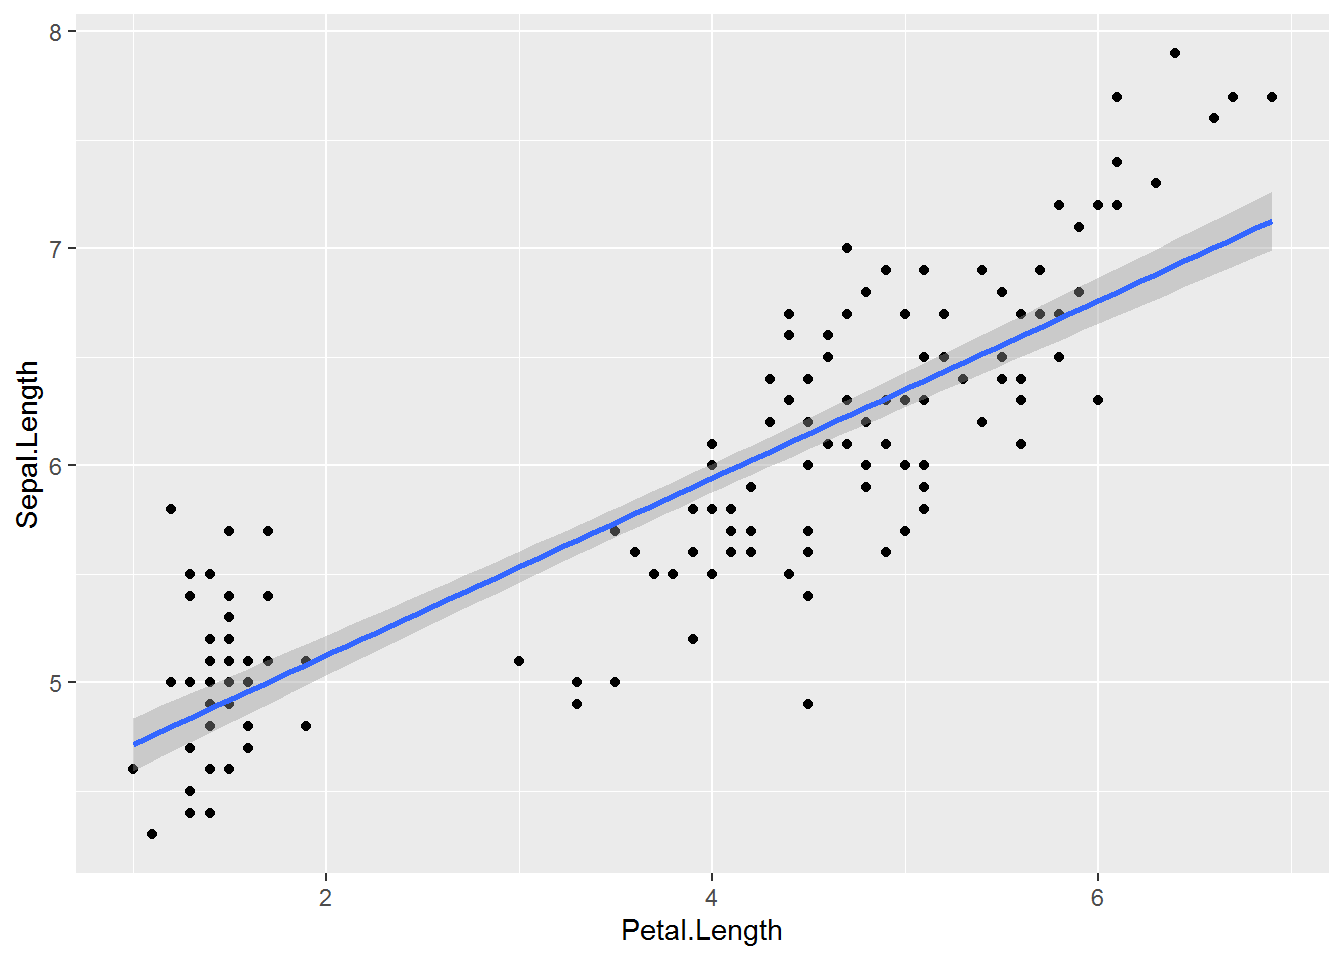
\includegraphics{introR_files/figure-latex/unnamed-chunk-27-1.pdf}

\begin{quote}
\hypertarget{ejercicio-3}{%
\subsection{Ejercicio:}\label{ejercicio-3}}

Discuta e interprete los coeficientes del modelo.
\end{quote}

Ahora utilizaremos el modelo que hemos calculado para predecir cómo se comporta la longitud del sépalo cuando la longitud del pétalo esta entre 2 y 4.

\begin{Shaded}
\begin{Highlighting}[]
\NormalTok{newdato <-}\StringTok{ }\KeywordTok{data.frame}\NormalTok{ (}\DataTypeTok{Petal.Length =} \KeywordTok{seq}\NormalTok{ (}\DecValTok{2}\NormalTok{, }\DecValTok{4}\NormalTok{, }\DataTypeTok{by =} \FloatTok{0.1}\NormalTok{))}
\KeywordTok{predict}\NormalTok{(model1, }\DataTypeTok{newdata =}\NormalTok{ newdato) }\CommentTok{# predice sepalo cuando petalo es de 4 a 7}
\end{Highlighting}
\end{Shaded}

\begin{verbatim}
##        1        2        3        4        5        6        7        8 
## 5.124448 5.165340 5.206232 5.247125 5.288017 5.328909 5.369801 5.410694 
##        9       10       11       12       13       14       15       16 
## 5.451586 5.492478 5.533370 5.574262 5.615155 5.656047 5.696939 5.737831 
##       17       18       19       20       21 
## 5.778724 5.819616 5.860508 5.901400 5.942293
\end{verbatim}

\begin{quote}
\hypertarget{ejercicio-4}{%
\subsection{Ejercicio:}\label{ejercicio-4}}

Use el modelo para predecir el sépalo cuando el pétalo tiene un valor de 7 o mas
\end{quote}

\hypertarget{regresiuxf3n-lineal-con-2-o-muxe1s-predictores}{%
\section{Regresión lineal con 2 o más predictores}\label{regresiuxf3n-lineal-con-2-o-muxe1s-predictores}}

Ahora haremos las cosas un poco más complejas (sin que sean difíciles) para entender que sucede cuando hay dos o más predictores de la forma:

\begin{equation} 
y = \alpha +\beta_{1}\mathit{x} +\beta_{2}\mathit{x} +\epsilon,
  \label{eq:binom}
\end{equation}

Usaremos mas (+) para combinar efectos. Dos puntos (:) para interacciones A:B; y asterisco para efectos e interacciones, ej A*B = A+B+A:B

\begin{Shaded}
\begin{Highlighting}[]
\NormalTok{model1a <-}\StringTok{ }\KeywordTok{lm}\NormalTok{(Sepal.Length}\OperatorTok{~}\NormalTok{Petal.Length }\OperatorTok{*}\StringTok{ }\NormalTok{Petal.Width, }\DataTypeTok{data=}\NormalTok{iris)}
\KeywordTok{summary}\NormalTok{(model1a)}
\end{Highlighting}
\end{Shaded}

\begin{verbatim}
## 
## Call:
## lm(formula = Sepal.Length ~ Petal.Length * Petal.Width, data = iris)
## 
## Residuals:
##      Min       1Q   Median       3Q      Max 
## -1.00058 -0.25209  0.00766  0.21640  0.89542 
## 
## Coefficients:
##                          Estimate Std. Error t value Pr(>|t|)    
## (Intercept)               4.57717    0.11195  40.885  < 2e-16 ***
## Petal.Length              0.44168    0.06551   6.742 3.38e-10 ***
## Petal.Width              -1.23932    0.21937  -5.649 8.16e-08 ***
## Petal.Length:Petal.Width  0.18859    0.03357   5.617 9.50e-08 ***
## ---
## Signif. codes:  0 '***' 0.001 '**' 0.01 '*' 0.05 '.' 0.1 ' ' 1
## 
## Residual standard error: 0.3667 on 146 degrees of freedom
## Multiple R-squared:  0.8078, Adjusted R-squared:  0.8039 
## F-statistic: 204.5 on 3 and 146 DF,  p-value: < 2.2e-16
\end{verbatim}

\begin{Shaded}
\begin{Highlighting}[]
\KeywordTok{library}\NormalTok{(lattice)}
\NormalTok{newdato<-}\KeywordTok{expand.grid}\NormalTok{(}\KeywordTok{list}\NormalTok{(}\DataTypeTok{Petal.Length =} \KeywordTok{seq}\NormalTok{(}\DecValTok{4}\NormalTok{, }\DecValTok{7}\NormalTok{, }\DataTypeTok{length.out=}\DecValTok{100}\NormalTok{), }
                          \DataTypeTok{Petal.Width=}\KeywordTok{seq}\NormalTok{(}\DecValTok{1}\NormalTok{, }\FloatTok{2.5}\NormalTok{, }\DataTypeTok{length.out=}\DecValTok{100}\NormalTok{)))}
\NormalTok{newdato}\OperatorTok{$}\NormalTok{Sepal.Length<-}\KeywordTok{predict}\NormalTok{(model1a, }\DataTypeTok{newdata =}\NormalTok{ newdato) }\CommentTok{# predice sepalo con petalo de 4 a 7 y 1 a 2.5}

\KeywordTok{levelplot}\NormalTok{(Sepal.Length}\OperatorTok{~}\NormalTok{Petal.Length }\OperatorTok{+}\StringTok{ }\NormalTok{Petal.Width, }\DataTypeTok{data=}\NormalTok{newdato,}
  \DataTypeTok{xlab =} \StringTok{"Petal.Length"}\NormalTok{, }\DataTypeTok{ylab =} \StringTok{"Petal.Width"}\NormalTok{,}
  \DataTypeTok{main =} \StringTok{"Surface of Sepal.Length"}\NormalTok{)}
\end{Highlighting}
\end{Shaded}

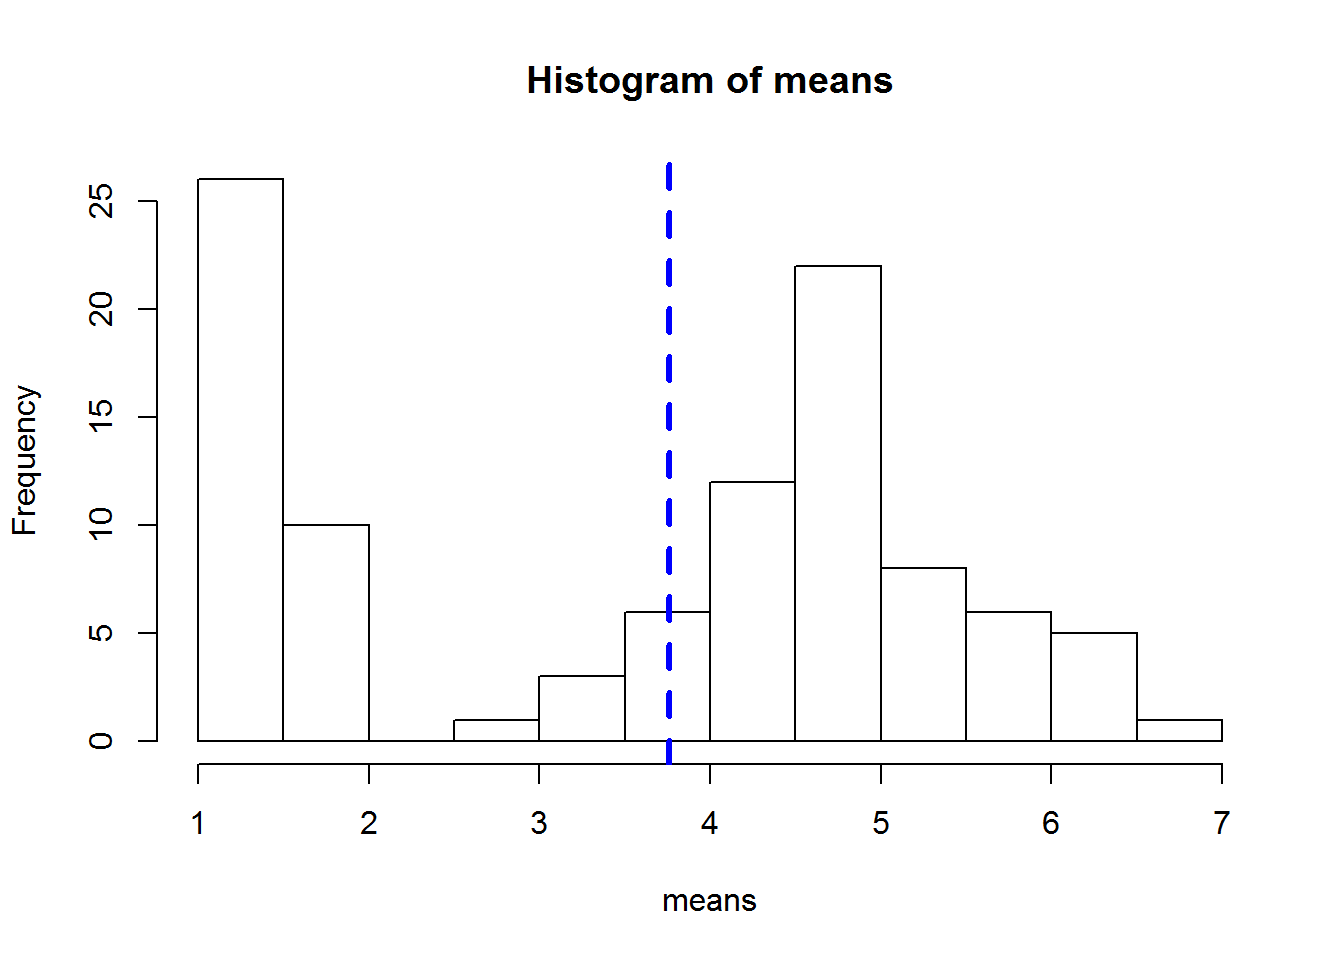
\includegraphics{introR_files/figure-latex/unnamed-chunk-29-1.pdf}

\begin{quote}
\hypertarget{ejercicio-5}{%
\subsection{Ejercicio:}\label{ejercicio-5}}

Cambie el rango de la predicción de 2 a 8
Cambie en el modelo la interacion de las covariables a +
\end{quote}

\hypertarget{modelos-de-distribuciuxf3n}{%
\chapter{Modelos de distribución}\label{modelos-de-distribuciuxf3n}}

En esta sección introduciremos algunos elementos matemáticos que no deben intimidarnos! Si bien las ecuaciones son aparentemente complejas el principio que hay detrás es muy elemental y se pude dominar mejor viendo los videos sugeridos.

\hypertarget{binomial}{%
\section{Binomial}\label{binomial}}

Recordemos la ecuación de la distribución Binomial:

\begin{equation} 
  P\left( x \right) = \frac{{n!}}{{k!\left( {n - k} \right)!}}p^k q^{n - k} = \left( {\begin{array}{*{20}c} n \\ k \\ \end{array}} \right)p^k q^{n - k}
  \label{eq:binom}
\end{equation}

Donde:
\(n\) es el número de ensayos.
\(k\) es el número de éxitos.
\(p\) es la probabilidad de exíto en un ensayo.
\(q=1-p\) es la probabilidad de fracasar en un ensayo.

Por favor \emph{no se asuste} por la aparente complejidad de la ecuación. Para simplificar la interpretación usaremos en lugar de la ecuación, el álgebra del modelo. Si desea aprender un poco mas de la distribución binomial le recomiendo el video que ha preparado \href{https://www.youtube.com/watch?v=sRoflgDiCKo}{Khan Academy.} con un interesante acento mexicano.

\begin{equation} 
  P\left( x \right) \sim \mathbf{Bin}(n,p)
  \label{eq:binom}
\end{equation}

\(P(x)\) es la probabilidad de un valor especifico de \(x\), el cual se distribuye de forma binomial \(Bin\) con los parámetros: \(n\) que corresponde al número de ensayos y \(p\) a la probabilidad.

A continuación, vamos a generar un set de \(n\) datos con una probabilidad dada \(p\). Estos datos son almacenados en un dataframe y luego visualizados como una distribución de frecuencias. La línea azul representa el promedio de esos datos.

\begin{Shaded}
\begin{Highlighting}[]
\NormalTok{n<-}\DecValTok{10} \CommentTok{# numero de datos}
\NormalTok{p<-}\StringTok{ }\FloatTok{0.5} \CommentTok{# probabilidad (~proporcion de unos)}
\CommentTok{# Generemos datos con esa informacion }
\NormalTok{daber<-}\KeywordTok{data.frame}\NormalTok{(}\DataTypeTok{estimado=}\KeywordTok{rbinom}\NormalTok{(n, }\DecValTok{1}\NormalTok{, p)) }
\CommentTok{# Grafiquemos }
\KeywordTok{library}\NormalTok{(ggplot2)}
\KeywordTok{ggplot}\NormalTok{(daber, }\KeywordTok{aes}\NormalTok{(}\DataTypeTok{x=}\NormalTok{estimado)) }\OperatorTok{+}\StringTok{ }
\StringTok{    }\KeywordTok{geom_histogram}\NormalTok{(}\KeywordTok{aes}\NormalTok{(}\DataTypeTok{y=}\NormalTok{..density..), }\CommentTok{# Histograma y densidad }
                   \DataTypeTok{binwidth=}\NormalTok{.}\DecValTok{1}\NormalTok{, }\CommentTok{# Ancho del bin}
                   \DataTypeTok{colour=}\StringTok{"black"}\NormalTok{, }\DataTypeTok{fill=}\StringTok{"white"}\NormalTok{) }\OperatorTok{+}\StringTok{ }
\StringTok{        }\KeywordTok{geom_vline}\NormalTok{(}\KeywordTok{aes}\NormalTok{(}\DataTypeTok{xintercept=}\KeywordTok{mean}\NormalTok{(estimado, }\DataTypeTok{na.rm=}\NormalTok{T)), }
          \DataTypeTok{color=}\StringTok{"blue"}\NormalTok{, }\DataTypeTok{linetype=}\StringTok{"dashed"}\NormalTok{, }\DataTypeTok{size=}\DecValTok{1}\NormalTok{) }\CommentTok{# media en azul}
\end{Highlighting}
\end{Shaded}

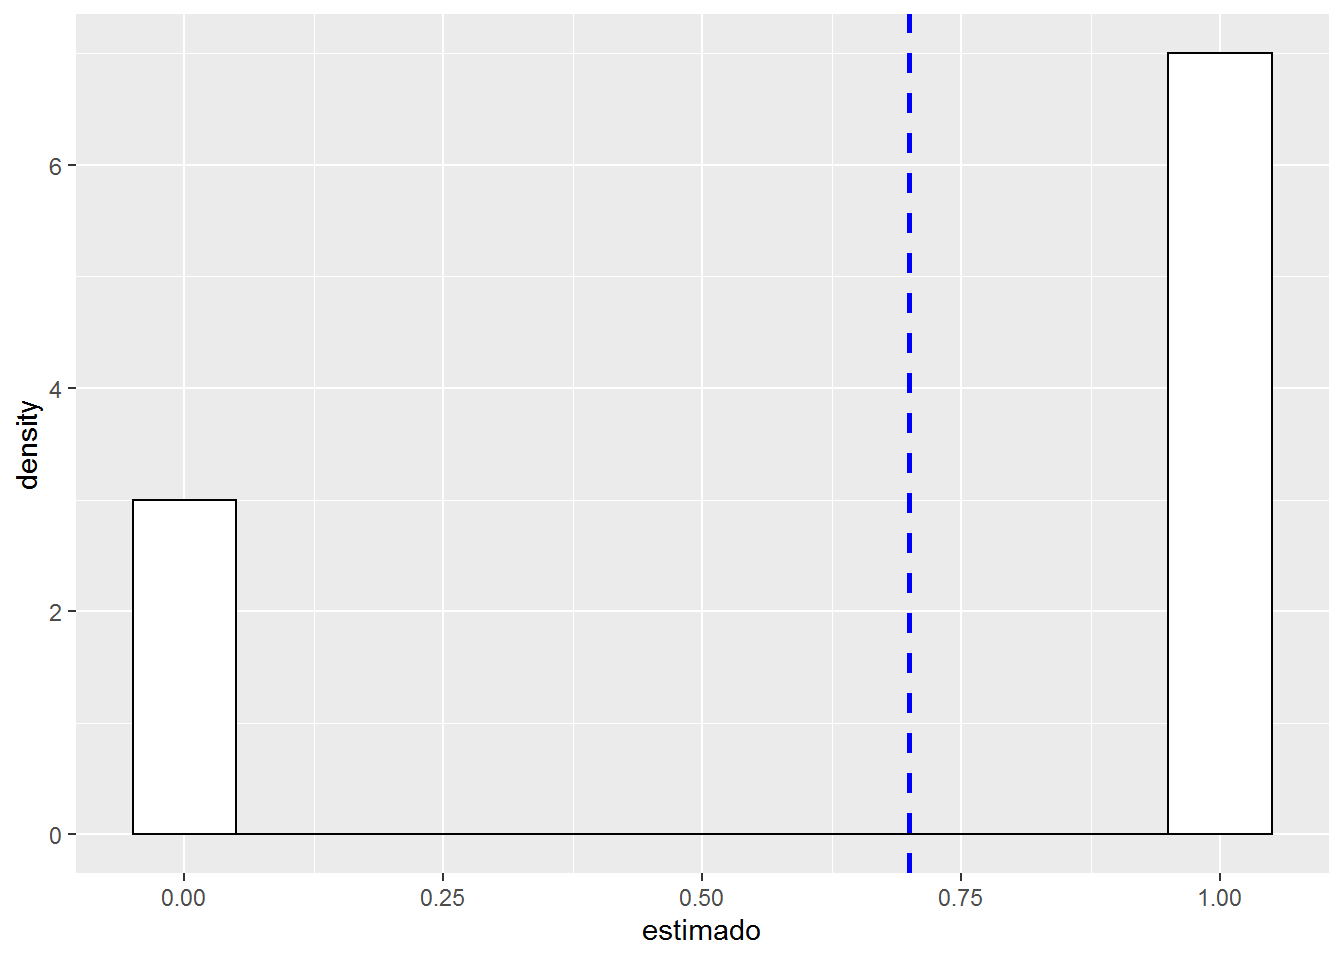
\includegraphics{introR_files/figure-latex/unnamed-chunk-30-1.pdf}

\begin{quote}
\hypertarget{ejercicio-6}{%
\subsection{Ejercicio:}\label{ejercicio-6}}

Varié primero el número de datos y luego la probabilidad haciéndola cercana a cero y luego cercana a uno. Vea como cambia el promedio con el número de datos y la probabilidad.
\end{quote}

\hypertarget{poisson}{%
\section{Poisson}\label{poisson}}

Recordemos la ecuación de la distribución Binomial:

\begin{equation} 
  P\left( x \right) = \frac{{e^{ - \mu } \mu ^x }}{{x!}}
  \label{eq:binom}
\end{equation}

Donde:

\(\mu\) es el número medio de ocurrencia (éxitos) en un intervalo en particular.
\(e\) es la constante 2.71828 (base of the Naperian logarithmic system).
\(x\) es el numero de ocurrencias (éxitos).
\(P(x)\) es la probabilidad de un valor especifico de \(x\).

De igual forma que en la distribución binomial, no nos dejemos intimidar por la complejidad de la ecuación y usemos el algebra del modelo que es mucho más sencilla. Si desea entender un poco mejor el proceso Poisson vean el video que preparo \href{https://www.youtube.com/watch?v=Vhjiw8r8kR4}{Khan Academy.}

\begin{equation} 
  P\left( x \right) \sim \mathbf{Pois}(\lambda)
  \label{eq:binom}
\end{equation}

Donde:

\(P(x)\) es la probabilidad de un valor especifico de \(x\), el cual se distribuye de acuerdo a la distribución Poisson (\(Pois\)) y que equivaldría a un valor específico del conteo.
\(\lambda\) es la media de la distribución.

\begin{Shaded}
\begin{Highlighting}[]
\NormalTok{n <-}\StringTok{ }\DecValTok{100}
\NormalTok{lambda <-}\StringTok{ }\DecValTok{10}
\NormalTok{poisson_data <-}\StringTok{ }\KeywordTok{data.frame}\NormalTok{(}\StringTok{'data'}\NormalTok{ =}\StringTok{ }\KeywordTok{rpois}\NormalTok{(n, lambda))}


\KeywordTok{library}\NormalTok{(tidyverse)}
\NormalTok{poisson_data }\OperatorTok\StringTok{ }\KeywordTok{ggplot}\NormalTok{() }\OperatorTok{+}\StringTok{ }
\StringTok{  }\KeywordTok{geom_histogram}\NormalTok{(}\KeywordTok{aes}\NormalTok{(}\DataTypeTok{x =}\NormalTok{ data, }
                     \DataTypeTok{y =} \KeywordTok{stat}\NormalTok{(count }\OperatorTok{/}\StringTok{ }\KeywordTok{sum}\NormalTok{(count))), }
                     \DataTypeTok{color =} \StringTok{'black'}\NormalTok{,}
                 \DataTypeTok{binwidth =} \DecValTok{1}\NormalTok{) }\OperatorTok{+}
\StringTok{  }\KeywordTok{geom_vline}\NormalTok{(}\DataTypeTok{xintercept =}\NormalTok{ lambda, }
             \DataTypeTok{size =} \DecValTok{1}\NormalTok{, }
             \DataTypeTok{linetype =} \StringTok{'dashed'}\NormalTok{,}
             \DataTypeTok{color =} \StringTok{'red'}\NormalTok{) }\OperatorTok{+}
\StringTok{  }\KeywordTok{theme_bw}\NormalTok{() }\OperatorTok{+}
\StringTok{  }\KeywordTok{labs}\NormalTok{(}\DataTypeTok{x =} \StringTok{'Number of successes per period'}\NormalTok{,}
       \DataTypeTok{y =} \StringTok{'Proportion'}\NormalTok{,}
       \DataTypeTok{title =} \StringTok{'1,000 samples of Pois(lambda = 10)'}\NormalTok{)}
\end{Highlighting}
\end{Shaded}

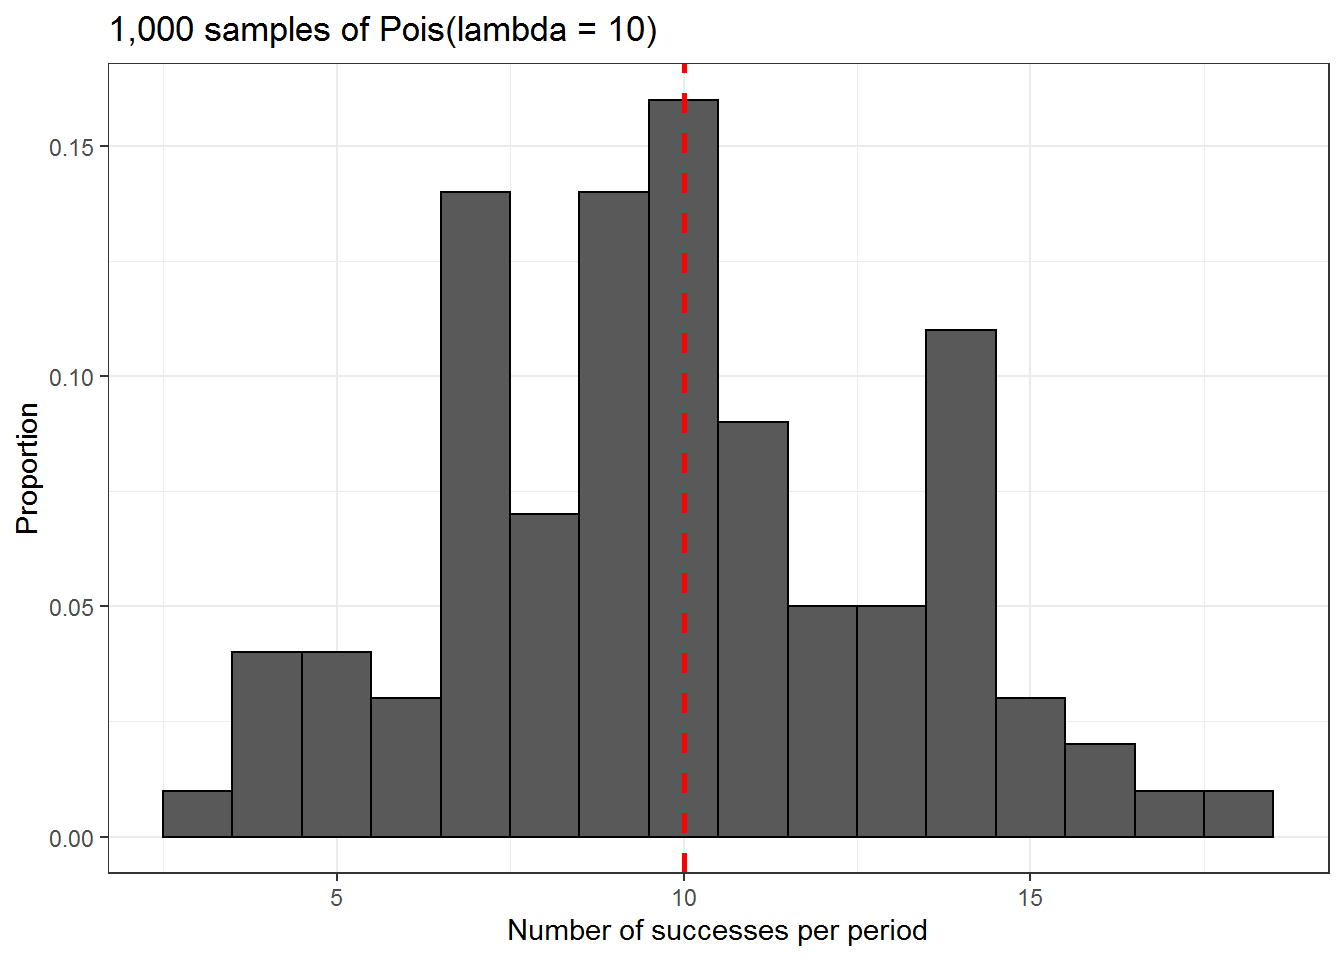
\includegraphics{introR_files/figure-latex/unnamed-chunk-31-1.pdf}

\begin{quote}
\hypertarget{ejercicio-7}{%
\subsection{Ejercicio:}\label{ejercicio-7}}

Use el modelo para variar n y lambda\ldots{} vea que sucede.
\end{quote}

  \bibliography{book.bib,packages.bib}

\end{document}
